\section{Задание №7}\label{07-lab}

\subsection{Условие}\label{07-lab-condition}

Придумать задачу коммивояжера размерности $10 \times 10$. Значения в матрице расстояний должны быть любыми целыми числами от 1 до 100.

Решить задачу методом ветвей и границ. Полный перебор не использовать.

После выполнения задания добавить в отчёт граф решения, добавить решение задачи с помощью программных средств.

\subsection{Постановка задачи}\label{07-lab-statement}

$n = 10$ городов. $c_{ij}$ - стоимость переезда из города $i$ в город $j$. $i, j = \overline{1, n}, i \neq j$.


\[
    C = \begin{pmatrix}
        \infty & 92     & 14     & 71     & 60     & 20     & 82     & 86     & 74     & 74     \\
        87     & \infty & 23     & 2      & 21     & 52     & 1      & 87     & 29     & 37     \\
        1      & 63     & \infty & 20     & 32     & 75     & 57     & 21     & 88     & 48     \\
        90     & 58     & 41     & \infty & 59     & 79     & 14     & 61     & 61     & 46     \\
        61     & 50     & 54     & 63     & \infty & 100    & 50     & 6      & 20     & 72     \\
        38     & 17     & 3      & 88     & 59     & \infty & 8      & 89     & 52     & 1      \\
        83     & 91     & 59     & 70     & 43     & 7      & \infty & 34     & 77     & 80     \\
        35     & 49     & 3      & 1      & 5      & 53     & 3      & \infty & 92     & 62     \\
        17     & 89     & 43     & 33     & 73     & 61     & 99     & 13     & \infty & 47     \\
        14     & 71     & 77     & 86     & 61     & 39     & 84     & 79     & 81     & \infty
    \end{pmatrix}
\]

$ x_{ij} = \begin{cases}
        1, & \text{если коммивояжер едет из i в j}, \\
        0, & \text{иначе}.
    \end{cases} $

Математическая модель задачи коммивояжера:

$ F = \sum\limits_{i=1}^{n} \sum\limits_{j=1}^{n} c_{ij} x_{ij} \to \min $

\[
    \begin{cases}
        \sum\limits_{j=1}^{n} x_{ij} = 1, i = \overline{1, n} \text{-- выезжает из каждого города ровно один раз} \\
        \sum\limits_{i=1}^{n} x_{ij} = 1, j = \overline{1, n} \text{-- въезжает в каждый город ровно один раз}    \\
        \text{Маршрут замкнут, петли отсутствуют}
    \end{cases}
\]

\subsection{Решение}\label{07-lab-solution}

Для начала заведём таблицу для решения задачи методом ветвей и границ.

\[
    \begin{array}{|>{\columncolor{lightgray}}c|c|c|c|c|c|c|c|c|c|c|>{\columncolor{LightBlue}}c|}
        \hline \rowcolor{lightgray}
        \text{Город} & 1      & 2      & 3      & 4      & 5      & 6      & 7      & 8      & 9      & 10     & \text{min}            \\
        \hline
        1            & \infty & 92     & 14     & 71     & 60     & 20     & 82     & 86     & 74     & 74     &                       \\
        \hline
        2            & 87     & \infty & 23     & 2      & 21     & 52     & 1      & 87     & 29     & 37     &                       \\
        \hline
        3            & 1      & 63     & \infty & 20     & 32     & 75     & 57     & 21     & 88     & 48     &                       \\
        \hline
        4            & 90     & 58     & 41     & \infty & 59     & 79     & 14     & 61     & 61     & 46     &                       \\
        \hline
        5            & 61     & 50     & 54     & 63     & \infty & 100    & 50     & 6      & 20     & 72     &                       \\
        \hline
        6            & 38     & 17     & 3      & 88     & 59     & \infty & 8      & 89     & 52     & 1      &                       \\
        \hline
        7            & 83     & 91     & 59     & 70     & 43     & 7      & \infty & 34     & 77     & 80     &                       \\
        \hline
        8            & 35     & 49     & 3      & 1      & 5      & 53     & 3      & \infty & 92     & 62     &                       \\
        \hline
        9            & 17     & 89     & 43     & 33     & 73     & 61     & 99     & 13     & \infty & 47     &                       \\
        \hline
        10           & 14     & 71     & 77     & 86     & 61     & 39     & 84     & 79     & 81     & \infty &                       \\
        \hline \rowcolor{LightBlue}
        \text{min}   &        &        &        &        &        &        &        &        &        &        & \cellcolor{Chocolate} \\
        \hline
    \end{array}
\]

Начинаем редуцировать таблицу. Для этого вычтем минимальный элемент в каждой строке из всех элементов строки. Далее вычтем минимальный элемент в каждом столбце из всех элементов столбца.
Таким образом мы получим редуцированную таблицу.

Расставим минимумы в каждой строке:

\[
    \begin{array}{|>{\columncolor{lightgray}}c|c|c|c|c|c|c|c|c|c|c|>{\columncolor{LightBlue}}c|}
        \hline \rowcolor{lightgray}
        \text{Город} & 1      & 2      & 3      & 4      & 5      & 6      & 7      & 8      & 9      & 10     & \text{min}            \\
        \hline
        1            & \infty & 92     & 14     & 71     & 60     & 20     & 82     & 86     & 74     & 74     & 14                    \\
        \hline
        2            & 87     & \infty & 23     & 2      & 21     & 52     & 1      & 87     & 29     & 37     & 1                     \\
        \hline
        3            & 1      & 63     & \infty & 20     & 32     & 75     & 57     & 21     & 88     & 48     & 1                     \\
        \hline
        4            & 90     & 58     & 41     & \infty & 59     & 79     & 14     & 61     & 61     & 46     & 14                    \\
        \hline
        5            & 61     & 50     & 54     & 63     & \infty & 100    & 50     & 6      & 20     & 72     & 6                     \\
        \hline
        6            & 38     & 17     & 3      & 88     & 59     & \infty & 8      & 89     & 52     & 1      & 1                     \\
        \hline
        7            & 83     & 91     & 59     & 70     & 43     & 7      & \infty & 34     & 77     & 80     & 7                     \\
        \hline
        8            & 35     & 49     & 3      & 1      & 5      & 53     & 3      & \infty & 92     & 62     & 1                     \\
        \hline
        9            & 17     & 89     & 43     & 33     & 73     & 61     & 99     & 13     & \infty & 47     & 13                    \\
        \hline
        10           & 14     & 71     & 77     & 86     & 61     & 39     & 84     & 79     & 81     & \infty & 14                    \\
        \hline \rowcolor{LightBlue}
        \text{min}   &        &        &        &        &        &        &        &        &        &        & \cellcolor{Chocolate} \\
        \hline
    \end{array}
\]

Вычтем минимальный элемент в каждой строке из всех элементов строки:

\[
    \begin{array}{|>{\columncolor{lightgray}}c|c|c|c|c|c|c|c|c|c|c|>{\columncolor{LightBlue}}c|}
        \hline \rowcolor{lightgray}
        \text{Город} & 1      & 2      & 3      & 4      & 5      & 6      & 7      & 8      & 9      & 10     & \text{min}            \\
        \hline
        1            & \infty & 78     & 0      & 57     & 46     & 6      & 68     & 72     & 60     & 60     & 14                    \\
        \hline
        2            & 86     & \infty & 22     & 1      & 20     & 51     & 0      & 86     & 28     & 36     & 1                     \\
        \hline
        3            & 0      & 62     & \infty & 19     & 31     & 74     & 56     & 20     & 87     & 47     & 1                     \\
        \hline
        4            & 76     & 44     & 27     & \infty & 45     & 65     & 0      & 47     & 47     & 32     & 14                    \\
        \hline
        5            & 55     & 44     & 48     & 57     & \infty & 94     & 44     & 0      & 14     & 66     & 6                     \\
        \hline
        6            & 37     & 16     & 2      & 87     & 58     & \infty & 7      & 88     & 51     & 0      & 1                     \\
        \hline
        7            & 76     & 84     & 52     & 63     & 36     & 0      & \infty & 27     & 70     & 73     & 7                     \\
        \hline
        8            & 34     & 48     & 2      & 0      & 4      & 52     & 2      & \infty & 91     & 61     & 1                     \\
        \hline
        9            & 4      & 76     & 30     & 20     & 60     & 48     & 86     & 0      & \infty & 34     & 13                    \\
        \hline
        10           & 0      & 57     & 63     & 72     & 47     & 25     & 70     & 65     & 67     & \infty & 14                    \\
        \hline \rowcolor{LightBlue}
        \text{min}   &        &        &        &        &        &        &        &        &        &        & \cellcolor{Chocolate} \\
        \hline
    \end{array}
\]

Расставим минимумы в каждом столбце:

\[
    \begin{array}{|>{\columncolor{lightgray}}c|c|c|c|c|c|c|c|c|c|c|>{\columncolor{LightBlue}}c|}
        \hline \rowcolor{lightgray}
        \text{Город} & 1      & 2      & 3      & 4      & 5      & 6      & 7      & 8      & 9      & 10     & \text{min}            \\
        \hline
        1            & \infty & 78     & 0      & 57     & 46     & 6      & 68     & 72     & 60     & 60     & 14                    \\
        \hline
        2            & 86     & \infty & 22     & 1      & 20     & 51     & 0      & 86     & 28     & 36     & 1                     \\
        \hline
        3            & 0      & 62     & \infty & 19     & 31     & 74     & 56     & 20     & 87     & 47     & 1                     \\
        \hline
        4            & 76     & 44     & 27     & \infty & 45     & 65     & 0      & 47     & 47     & 32     & 14                    \\
        \hline
        5            & 55     & 44     & 48     & 57     & \infty & 94     & 44     & 0      & 14     & 66     & 6                     \\
        \hline
        6            & 37     & 16     & 2      & 87     & 58     & \infty & 7      & 88     & 51     & 0      & 1                     \\
        \hline
        7            & 76     & 84     & 52     & 63     & 36     & 0      & \infty & 27     & 70     & 73     & 7                     \\
        \hline
        8            & 34     & 48     & 2      & 0      & 4      & 52     & 2      & \infty & 91     & 61     & 1                     \\
        \hline
        9            & 4      & 76     & 30     & 20     & 60     & 48     & 86     & 0      & \infty & 34     & 13                    \\
        \hline
        10           & 0      & 57     & 63     & 72     & 47     & 25     & 70     & 65     & 67     & \infty & 14                    \\
        \hline \rowcolor{LightBlue}
        \text{min}   & 0      & 16     & 0      & 0      & 4      & 0      & 0      & 0      & 14     & 0      & \cellcolor{Chocolate} \\
        \hline
    \end{array}
\]

Вычтем минимальный элемент в каждом столбце из всех элементов столбца:

\[
    \begin{array}{|>{\columncolor{lightgray}}c|c|c|c|c|c|c|c|c|c|c|>{\columncolor{LightBlue}}c|}
        \hline \rowcolor{lightgray}
        \text{Город} & 1      & 2      & 3      & 4      & 5      & 6      & 7      & 8      & 9      & 10     & \text{min}            \\
        \hline
        1            & \infty & 62     & 0      & 57     & 42     & 6      & 68     & 72     & 46     & 60     & 14                    \\
        \hline
        2            & 86     & \infty & 22     & 1      & 16     & 51     & 0      & 86     & 14     & 36     & 1                     \\
        \hline
        3            & 0      & 46     & \infty & 19     & 27     & 74     & 56     & 20     & 73     & 47     & 1                     \\
        \hline
        4            & 76     & 28     & 27     & \infty & 41     & 65     & 0      & 47     & 33     & 32     & 14                    \\
        \hline
        5            & 55     & 28     & 48     & 57     & \infty & 94     & 44     & 0      & 0      & 66     & 6                     \\
        \hline
        6            & 37     & 0      & 2      & 87     & 54     & \infty & 7      & 88     & 37     & 0      & 1                     \\
        \hline
        7            & 76     & 68     & 52     & 63     & 32     & 0      & \infty & 27     & 56     & 73     & 7                     \\
        \hline
        8            & 34     & 32     & 2      & 0      & 0      & 52     & 2      & \infty & 77     & 61     & 1                     \\
        \hline
        9            & 4      & 60     & 30     & 20     & 56     & 48     & 86     & 0      & \infty & 34     & 13                    \\
        \hline
        10           & 0      & 41     & 63     & 72     & 43     & 25     & 70     & 65     & 53     & \infty & 14                    \\
        \hline \rowcolor{LightBlue}
        \text{min}   & 0      & 16     & 0      & 0      & 4      & 0      & 0      & 0      & 14     & 0      & \cellcolor{Chocolate} \\
        \hline
    \end{array}
\]

Будем обозначать за $h$ сумму приводящих элементов, то есть сумму элементов в строке и столбце $min$. $h = 14 + 1 + 1 + 14 + 6 + 1 + 7 + 1 + 13 + 14 + 0 + 16 + 0 + 4 + 0 + 0 + 0 + 14 + 0 = 106$.

\[
    \begin{array}{|>{\columncolor{lightgray}}c|c|c|c|c|c|c|c|c|c|c|>{\columncolor{LightBlue}}c|}
        \hline \rowcolor{lightgray}
        \text{Город} & 1      & 2      & 3      & 4      & 5      & 6      & 7      & 8      & 9      & 10     & \text{min}                \\
        \hline
        1            & \infty & 62     & 0      & 57     & 42     & 6      & 68     & 72     & 46     & 60     & 14                        \\
        \hline
        2            & 86     & \infty & 22     & 1      & 16     & 51     & 0      & 86     & 14     & 36     & 1                         \\
        \hline
        3            & 0      & 46     & \infty & 19     & 27     & 74     & 56     & 20     & 73     & 47     & 1                         \\
        \hline
        4            & 76     & 28     & 27     & \infty & 41     & 65     & 0      & 47     & 33     & 32     & 14                        \\
        \hline
        5            & 55     & 28     & 48     & 57     & \infty & 94     & 44     & 0      & 0      & 66     & 6                         \\
        \hline
        6            & 37     & 0      & 2      & 87     & 54     & \infty & 7      & 88     & 37     & 0      & 1                         \\
        \hline
        7            & 76     & 68     & 52     & 63     & 32     & 0      & \infty & 27     & 56     & 73     & 7                         \\
        \hline
        8            & 34     & 32     & 2      & 0      & 0      & 52     & 2      & \infty & 77     & 61     & 1                         \\
        \hline
        9            & 4      & 60     & 30     & 20     & 56     & 48     & 86     & 0      & \infty & 34     & 13                        \\
        \hline
        10           & 0      & 41     & 63     & 72     & 43     & 25     & 70     & 65     & 53     & \infty & 14                        \\
        \hline \rowcolor{LightBlue}
        \text{min}   & 0      & 16     & 0      & 0      & 4      & 0      & 0      & 0      & 14     & 0      & \cellcolor{Chocolate} 106 \\
        \hline
    \end{array}
\]

Это значит, что решение задачи коммивояжера на данном этапе нельзя решить менее чем за $h = 106$ единиц.
Сейчас множество допустимых решений --- $G_0$. На данном этапе это множество всех полных циклов без петель, которые можно построить на графе, так как мы ещё не выкидывали неоптимальные ветви.

То есть оценка множеств допустимых решений $w(G_0) = 106$.

Выбираем претендентов на ветвление. Претендент на ветвление --- это элемент матрицы, равный нулю.
Записываем претендентов на ветвление в таблицу. Строка $S$ --- это строка, в которой находится претендент на ветвление.
Строки $d_i$ и $d_j$ --- это минимальные элементы по строке и столбцу, в которых находится претендент на ветвление (если не учитывать самого претендента на ветвление).
Строка $Q_{ij}$ --- это $d_i + d_j$.

\[
    \begin{array}{|>{\columncolor{lightgray}}c|c|c|c|c|c|c|c|c|c|c|c|c|c|}
        \hline
        S      & (1,3) & (2, 7) & (3, 1) & (4, 7) & (5, 8) & (5, 9) & (6, 2) & (6, 10) & (7, 6) & (8, 4) & (8, 5) & (9, 8) & (10, 1) \\
        \hline
        d_i    & 6     & 1      & 19     & 27     & 0      & 0      & 0      & 0       & 27     & 0      & 0      & 4      & 25      \\
        \hline
        d_j    & 2     & 0      & 0      & 0      & 0      & 14     & 28     & 32      & 6      & 1      & 16     & 0      & 0       \\
        \hline
        Q_{ij} & 8     & 1      & 19     & 27     & 0      & 14     & 28     & 32      & 33     & 1      & 16     & 4      & 25      \\
        \hline
    \end{array}
\]

$\max Q_{ij} = Q_{7, 6} = 33$. Ветвление производим по элементу $(7, 6)$. Начинаем строить дерево ветвей. Либо коммивояжер едет из 7 в 6, либо нет.

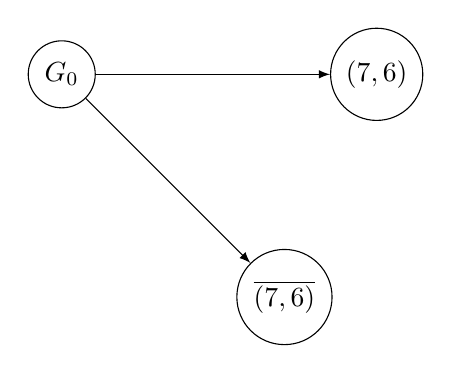
\begin{tikzpicture}[
        grow=east, % Дерево растет слева направо
        level 1/.style = {level distance=4cm}, % Расстояние между уровнями
        edge from parent/.style = {draw, -latex},
        kant/.style={text width=2cm, text centered, sloped},
        cell/.style={circle, draw, align=center}, % Стиль узлов
    ]

    \node[cell] {$G_0$}
    child[grow=east] {node[cell] {$(7, 6)$}}
    child[grow=south east] {node[cell] {$\overline{(7, 6)}$}};

\end{tikzpicture}

Будем обозначать $(i, j)$ или $\overline{(i, j)}$ за множество допустимых решений, где мы выбрали или не выбрали переезд из города $i$ в город $j$.

Найдём оценку множества $\overline{(7, 6)}$: $w(\overline{(7, 6)}) = w(G_0) + Q_{7, 6} = 106 + 33 = 139$. То есть стоимость не взять переезд из 10 в 1 увеличит стоимость на 33 единицы.

Найдём оценку множества $(7, 6)$. Для этого нужно вычеркнуть из таблицы строку 7 и столбец 6, а также исключить циклы: поставить $\infty$ в ячейку $(6, 7)$, чтобы не возникло цикла $7 \to 6 \to 7$.

\[
    \begin{array}{|>{\columncolor{lightgray}}c|c|c|c|c|c|c|c|c|c|>{\columncolor{LightBlue}}c|}
        \hline \rowcolor{lightgray}
        \text{Город} & 1      & 2      & 3      & 4      & 5      & 7      & 8      & 9      & 10     & \text{min}            \\
        \hline
        1            & \infty & 62     & 0      & 57     & 42     & 68     & 72     & 46     & 60     &                       \\
        \hline
        2            & 86     & \infty & 22     & 1      & 16     & 0      & 86     & 14     & 36     &                       \\
        \hline
        3            & 0      & 46     & \infty & 19     & 27     & 56     & 20     & 73     & 47     &                       \\
        \hline
        4            & 76     & 28     & 27     & \infty & 41     & 0      & 47     & 33     & 32     &                       \\
        \hline
        5            & 55     & 28     & 48     & 57     & \infty & 44     & 0      & 0      & 66     &                       \\
        \hline
        6            & 37     & 0      & 2      & 87     & 54     & \infty & 88     & 37     & 0      &                       \\
        \hline
        8            & 34     & 32     & 2      & 0      & 0      & 2      & \infty & 77     & 61     &                       \\
        \hline
        9            & 4      & 60     & 30     & 20     & 56     & 86     & 0      & \infty & 34     &                       \\
        \hline
        10           & 0      & 41     & 63     & 72     & 43     & 70     & 65     & 53     & \infty &                       \\
        \hline \rowcolor{LightBlue}
        \text{min}   &        &        &        &        &        &        &        &        &        & \cellcolor{Chocolate} \\
        \hline
    \end{array}
\]

Редуцируем матрицу и находим $h$:

\[
    \begin{array}{|>{\columncolor{lightgray}}c|c|c|c|c|c|c|c|c|c|>{\columncolor{LightBlue}}c|}
        \hline \rowcolor{lightgray}
        \text{Город} & 1      & 2      & 3      & 4      & 5      & 7      & 8      & 9      & 10     & \text{min}             \\
        \hline
        1            & \infty & 62     & 0      & 57     & 42     & 68     & 72     & 46     & 60     & 0                      \\
        \hline
        2            & 86     & \infty & 22     & 1      & 16     & 0      & 86     & 14     & 36     & 0                      \\
        \hline
        3            & 0      & 46     & \infty & 19     & 27     & 56     & 20     & 73     & 47     & 0                      \\
        \hline
        4            & 76     & 28     & 27     & \infty & 41     & 0      & 47     & 33     & 32     & 0                      \\
        \hline
        5            & 55     & 28     & 48     & 57     & \infty & 44     & 0      & 0      & 66     & 0                      \\
        \hline
        6            & 37     & 0      & 2      & 87     & 54     & \infty & 88     & 37     & 0      & 0                      \\
        \hline
        8            & 34     & 32     & 2      & 0      & 0      & 2      & \infty & 77     & 61     & 0                      \\
        \hline
        9            & 4      & 60     & 30     & 20     & 56     & 86     & 0      & \infty & 34     & 0                      \\
        \hline
        10           & 0      & 41     & 63     & 72     & 43     & 70     & 65     & 53     & \infty & 0                      \\
        \hline \rowcolor{LightBlue}
        \text{min}   & 0      & 0      & 0      & 0      & 0      & 0      & 0      & 0      & 0      & \cellcolor{Chocolate}0 \\
        \hline
    \end{array}
\]

$h = 0$. Это значит, что $w((7, 6)) = w(G_0) + h = 106 + 0 = 106$. То есть оценка множества $(7, 6)$ --- 106.

$w(\overline{(7, 6)}) = 139$, $w((7, 6)) = 106$. Выбираем ветвь с меньшей оценкой, то есть $(7, 6)$.

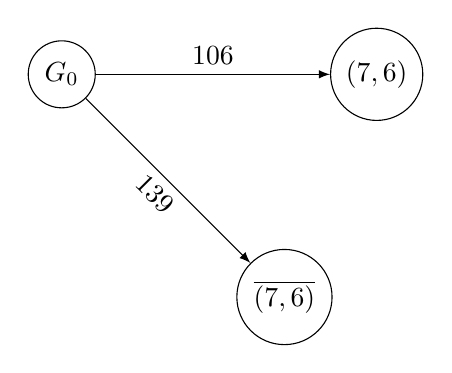
\begin{tikzpicture}[
        grow=east, % Дерево растет слева направо
        level 1/.style = {level distance=4cm}, % Расстояние между уровнями
        edge from parent/.style = {draw, -latex},
        kant/.style={text width=2cm, text centered, sloped},
        cell/.style={circle, draw, align=center}, % Стиль узлов
    ]

    \node[cell] {$G_0$}
    child[grow=east] {node[cell] {$(7, 6)$} edge from parent node[kant, above] {106}}
    child[grow=south east] {node[cell] {$\overline{(7, 6)}$} edge from parent node[kant, below] {139}};

\end{tikzpicture}

По последней таблице найдём претендентов на ветвление:

\[
    \begin{array}{|>{\columncolor{lightgray}}c|c|c|c|c|c|c|c|c|c|c|c|c|c|}
        \hline
        S      & (1,3) & (2, 7) & (3, 1) & (4, 7) & (5, 8) & (5, 9) & (6, 2) & (6, 10) & (8, 4) & (8, 5) & (9, 8) & (10, 1) \\
        \hline
        d_i    & 42    & 1      & 19     & 27     & 0      & 0      & 0      & 0       & 0      & 0      & 4      & 41      \\
        \hline
        d_j    & 2     & 0      & 0      & 0      & 0      & 14     & 28     & 32      & 1      & 16     & 0      & 0       \\
        \hline
        Q_{ij} & 44    & 1      & 19     & 27     & 0      & 14     & 28     & 32      & 1      & 16     & 4      & 41      \\
        \hline
    \end{array}
\]

$\max Q_{ij} = Q_{1, 3} = 44$. Ветвление производим по элементу $(1, 3)$.

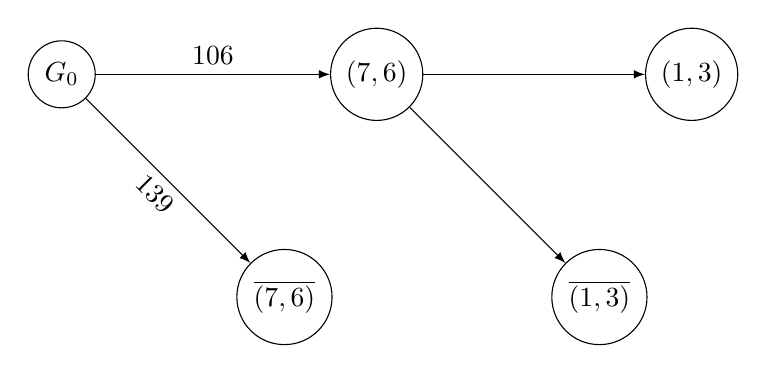
\begin{tikzpicture}[
        grow=east, % Дерево растет слева направо
        level 1/.style = {level distance=4cm}, % Расстояние между уровнями
        edge from parent/.style = {draw, -latex},
        kant/.style={text width=2cm, text centered, sloped},
        cell/.style={circle, draw, align=center}, % Стиль узлов
    ]

    \node[cell] {$G_0$}
    child[grow=east] {node[cell] {$(7, 6)$}
            child[grow=east] {node[cell] {$(1, 3)$}}
            child[grow=south east] {node[cell] {$\overline{(1, 3)}$}}
            edge from parent node[kant, above] {106}}
    child[grow=south east] {node[cell] {$\overline{(7, 6)}$} edge from parent node[kant, below] {139}};

\end{tikzpicture}

Найдём оценку множества $\overline{(1, 3)}$: $w(\overline{(1, 3)}) = w((7, 6)) + Q_{1, 3} = 106 + 44 = 150$.

Найдём оценку множества $(1, 3)$. Для этого нужно вычеркнуть из таблицы строку 1 и столбец 3, а также исключить циклы: поставить $\infty$ в ячейку $(3, 1)$, чтобы не возникло цикла $1 \to 3 \to 1$. Далее нужно редуцировать эту матрицу.

\[
    \begin{array}{|>{\columncolor{lightgray}}c|c|c|c|c|c|c|c|c|>{\columncolor{LightBlue}}c|}
        \hline \rowcolor{lightgray}
        \text{Город} & 1      & 2      & 4      & 5      & 7      & 8      & 9      & 10     & \text{min}              \\
        \hline
        2            & 86     & \infty & 1      & 16     & 0      & 86     & 14     & 36     & 0                       \\
        \hline
        3            & \infty & 27     & 0      & 8      & 37     & 1      & 54     & 28     & 19                      \\
        \hline
        4            & 76     & 28     & \infty & 41     & 0      & 47     & 33     & 32     & 0                       \\
        \hline
        5            & 55     & 28     & 57     & \infty & 44     & 0      & 0      & 66     & 0                       \\
        \hline
        6            & 37     & 0      & 87     & 54     & \infty & 88     & 37     & 0      & 0                       \\
        \hline
        8            & 34     & 32     & 0      & 0      & 2      & \infty & 77     & 61     & 0                       \\
        \hline
        9            & 4      & 60     & 20     & 56     & 86     & 0      & \infty & 34     & 0                       \\
        \hline
        10           & 0      & 41     & 72     & 43     & 70     & 65     & 53     & \infty & 0                       \\
        \hline \rowcolor{LightBlue}
        \text{min}   & 0      & 0      & 0      & 0      & 0      & 0      & 0      & 0      & \cellcolor{Chocolate}19 \\
        \hline
    \end{array}
\]

$h = 19$. Это значит, что $w((1, 3)) = w((7, 6)) + h = 106 + 19 = 125$.

$w(\overline{(1, 3)}) = 150$, $w((1, 3)) = 125$. Выбираем ветвь с меньшей оценкой, то есть $(1, 3)$.

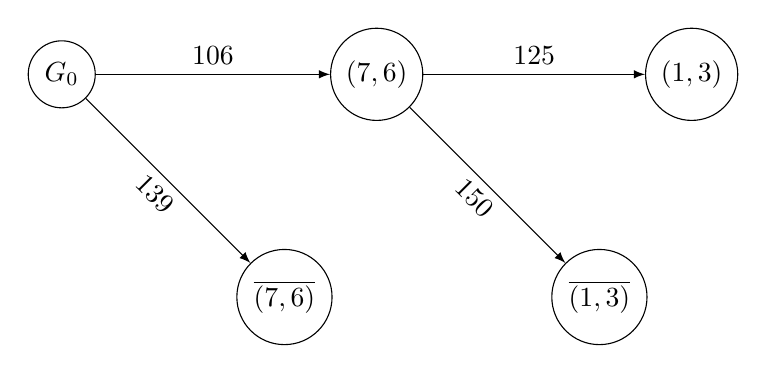
\begin{tikzpicture}[
        grow=east, % Дерево растет слева направо
        level 1/.style = {level distance=4cm}, % Расстояние между уровнями
        edge from parent/.style = {draw, -latex},
        kant/.style={text width=2cm, text centered, sloped},
        cell/.style={circle, draw, align=center}, % Стиль узлов
    ]

    \node[cell] {$G_0$}
    child[grow=east] {node[cell] {$(7, 6)$}
            child[grow=east] {node[cell] {$(1, 3)$} edge from parent node[kant, above] {125}}
            child[grow=south east] {node[cell] {$\overline{(1, 3)}$} edge from parent node[kant, below] {150}}
            edge from parent node[kant, above] {106}}
    child[grow=south east] {node[cell] {$\overline{(7, 6)}$} edge from parent node[kant, below] {139}};

\end{tikzpicture}

Найдём претендентов на ветвление:

\[
    \begin{array}{|>{\columncolor{lightgray}}c|c|c|c|c|c|c|c|c|c|c|c|c|c|}
        \hline
        S      & (2, 7) & (3, 4) & (4, 7) & (5, 8) & (5, 9) & (6, 2) & (6, 10) & (8, 4) & (8, 5) & (9, 8) & (10, 1) \\
        \hline
        d_i    & 1      & 1      & 28     & 0      & 0      & 0      & 0       & 0      & 0      & 4      & 41      \\
        \hline
        d_j    & 0      & 0      & 0      & 0      & 14     & 27     & 28      & 0      & 8      & 0      & 4       \\
        \hline
        Q_{ij} & 1      & 1      & 28     & 0      & 14     & 27     & 28      & 0      & 8      & 4      & 45      \\
        \hline
    \end{array}
\]

$\max Q_{ij} = Q_{10, 1} = 45$. Ветвление производим по элементу $(10, 1)$.

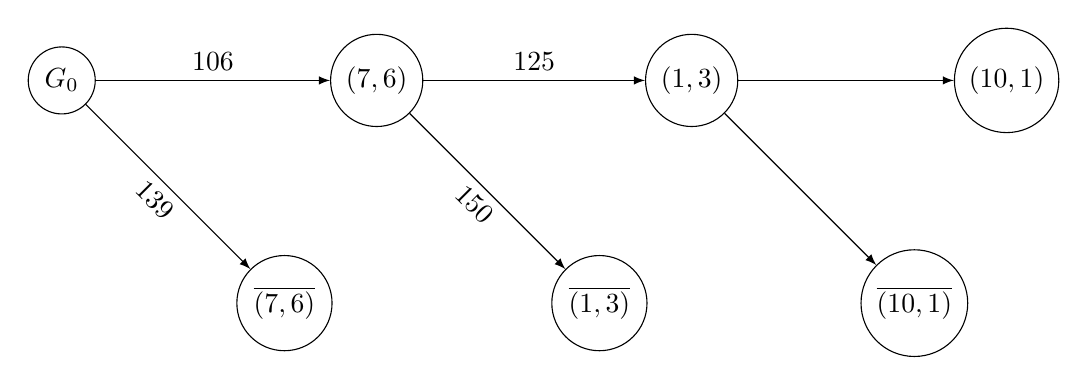
\begin{tikzpicture}[
        grow=east, % Дерево растет слева направо
        level 1/.style = {level distance=4cm}, % Расстояние между уровнями
        edge from parent/.style = {draw, -latex},
        kant/.style={text width=2cm, text centered, sloped},
        cell/.style={circle, draw, align=center}, % Стиль узлов
    ]

    \node[cell] {$G_0$}
    child[grow=east] {node[cell] {$(7, 6)$}
            child[grow=east] {node[cell] {$(1, 3)$}
                    child[grow=east] {node[cell] {$(10, 1)$}}
                    child[grow=south east] {node[cell] {$\overline{(10, 1)}$}}
                    edge from parent node[kant, above] {125}}
            child[grow=south east] {node[cell] {$\overline{(1, 3)}$} edge from parent node[kant, below] {150}}
            edge from parent node[kant, above] {106}}
    child[grow=south east] {node[cell] {$\overline{(7, 6)}$} edge from parent node[kant, below] {139}};

\end{tikzpicture}

Найдём оценку множества $\overline{(10, 1)}$: $w(\overline{(10, 1)}) = w((1, 3)) + Q_{10, 1} = 125 + 45 = 170$.

Найдём оценку множества $(10, 1)$. Для этого нужно вычеркнуть из таблицы строку 10 и столбец 1. Далее поставить $\infty$ в ячейку $(3, 10)$ чтобы не возникло цикла $1 \to 3 \to 10 \to 1$. И редуцировать эту таблицу.

\[
    \begin{array}{|>{\columncolor{lightgray}}c|c|c|c|c|c|c|c|>{\columncolor{LightBlue}}c|}
        \hline \rowcolor{lightgray}
        \text{Город} & 2      & 4      & 5      & 7      & 8      & 9      & 10     & \text{min}             \\
        \hline
        2            & \infty & 1      & 16     & 0      & 86     & 14     & 36     & 0                      \\
        \hline
        3            & 27     & 0      & 8      & 37     & 1      & 54     & \infty & 0                      \\
        \hline
        4            & 28     & \infty & 41     & 0      & 47     & 33     & 32     & 0                      \\
        \hline
        5            & 28     & 57     & \infty & 44     & 0      & 0      & 66     & 0                      \\
        \hline
        6            & 0      & 87     & 54     & \infty & 88     & 37     & 0      & 0                      \\
        \hline
        8            & 32     & 0      & 0      & 2      & \infty & 77     & 61     & 0                      \\
        \hline
        9            & 60     & 20     & 56     & 86     & 0      & \infty & 34     & 0                      \\
        \hline \rowcolor{LightBlue}
        \text{min}   & 0      & 0      & 0      & 0      & 0      & 0      & 0      & \cellcolor{Chocolate}0 \\
        \hline
    \end{array}
\]

$h = 0$. Это значит, что $w((10, 1)) = w((1, 3)) + h = 125 + 0 = 125$.

$w(\overline{(10, 1)}) = 170$, $w((10, 1)) = 125$. Выбираем ветвь с меньшей оценкой, то есть $(10, 1)$.

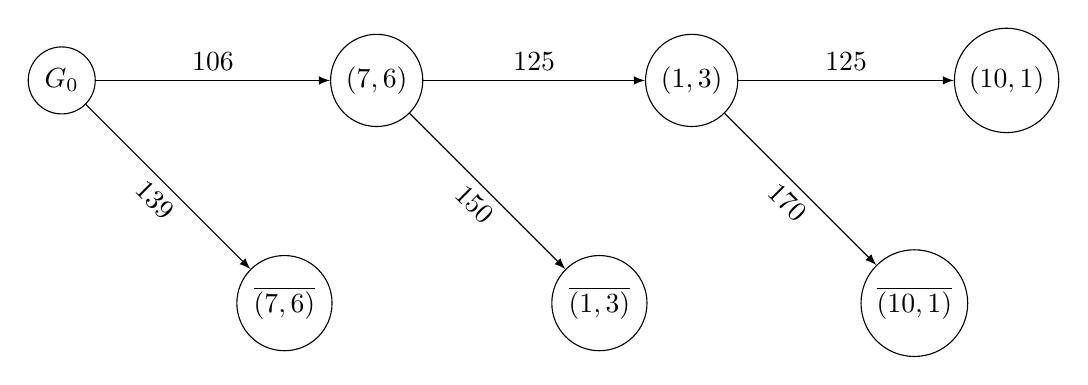
\begin{tikzpicture}[
        grow=east, % Дерево растет слева направо
        level 1/.style = {level distance=4cm}, % Расстояние между уровнями
        edge from parent/.style = {draw, -latex},
        kant/.style={text width=2cm, text centered, sloped},
        cell/.style={circle, draw, align=center}, % Стиль узлов
    ]

    \node[cell] {$G_0$}
    child[grow=east] {node[cell] {$(7, 6)$}
            child[grow=east] {node[cell] {$(1, 3)$}
                    child[grow=east] {node[cell] {$(10, 1)$} edge from parent node[kant, above] {125}}
                    child[grow=south east] {node[cell] {$\overline{(10, 1)}$} edge from parent node[kant, below] {170}}
                    edge from parent node[kant, above] {125}}
            child[grow=south east] {node[cell] {$\overline{(1, 3)}$} edge from parent node[kant, below] {150}}
            edge from parent node[kant, above] {106}}
    child[grow=south east] {node[cell] {$\overline{(7, 6)}$} edge from parent node[kant, below] {139}};

\end{tikzpicture}

Найдём претендентов на ветвление:

\[
    \begin{array}{|>{\columncolor{lightgray}}c|c|c|c|c|c|c|c|c|c|c|c|c|c|}
        \hline
        S      & (2, 7) & (3, 4) & (4, 7) & (5, 8) & (5, 9) & (6, 2) & (6, 10) & (8, 4) & (8, 5) & (9, 8) \\
        \hline
        d_i    & 1      & 1      & 28     & 0      & 0      & 0      & 0       & 0      & 0      & 20     \\
        \hline
        d_j    & 0      & 0      & 0      & 0      & 14     & 27     & 32      & 0      & 8      & 0      \\
        \hline
        Q_{ij} & 1      & 1      & 28     & 0      & 14     & 27     & 32      & 0      & 8      & 20     \\
        \hline
    \end{array}
\]

$\max Q_{ij} = Q_{6, 10} = 32$. Ветвление производим по элементу $(6, 10)$.

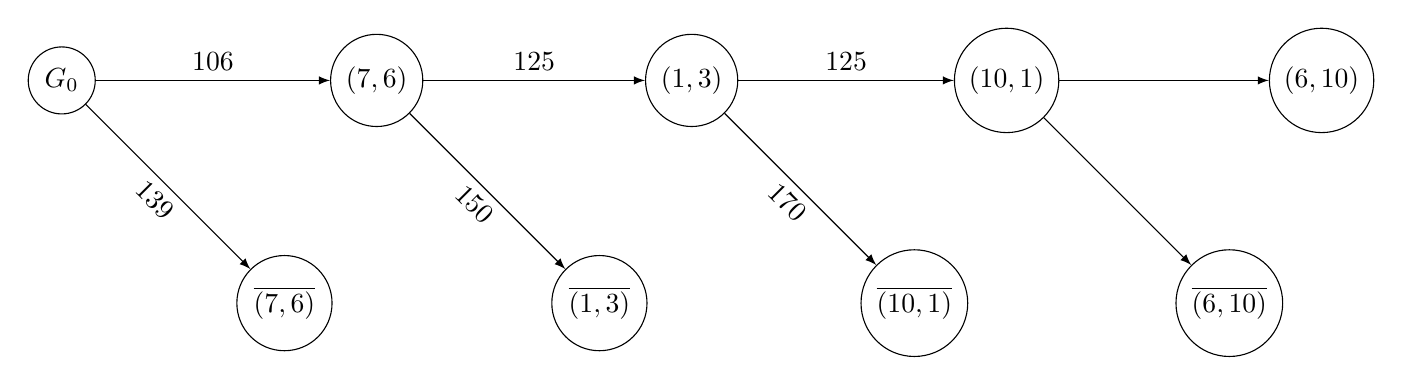
\begin{tikzpicture}[
        grow=east, % Дерево растет слева направо
        level 1/.style = {level distance=4cm}, % Расстояние между уровнями
        edge from parent/.style = {draw, -latex},
        kant/.style={text width=2cm, text centered, sloped},
        cell/.style={circle, draw, align=center}, % Стиль узлов
    ]

    \node[cell] {$G_0$}
    child[grow=east] {node[cell] {$(7, 6)$}
            child[grow=east] {node[cell] {$(1, 3)$}
                    child[grow=east] {node[cell] {$(10, 1)$}
                            child[grow=east] {node[cell] {$(6, 10)$}}
                            child[grow=south east] {node[cell] {$\overline{(6, 10)}$}}
                            edge from parent node[kant, above] {125}}
                    child[grow=south east] {node[cell] {$\overline{(10, 1)}$} edge from parent node[kant, below] {170}}
                    edge from parent node[kant, above] {125}}
            child[grow=south east] {node[cell] {$\overline{(1, 3)}$} edge from parent node[kant, below] {150}}
            edge from parent node[kant, above] {106}}
    child[grow=south east] {node[cell] {$\overline{(7, 6)}$} edge from parent node[kant, below] {139}};

\end{tikzpicture}

Находим оценку множества $\overline{(6, 10)}$: $w(\overline{(6, 10)}) = w((10, 1)) + Q_{6, 10} = 125 + 32 = 157$.

Находим оценку множества $(6, 10)$. Для этого нужно вычеркнуть из таблицы строку 6 и столбец 10, а также исключить циклы: поставить $\infty$ в ячейку $(3, 7)$, чтобы не возникло цикла $7 \to 6 \to 10 \to 1 \to 3 \to 7$. И редуцировать эту таблицу.

\[
    \begin{array}{|>{\columncolor{lightgray}}c|c|c|c|c|c|c|>{\columncolor{LightBlue}}c|}
        \hline \rowcolor{lightgray}
        \text{Город} & 2      & 4      & 5      & 7      & 8      & 9      & \text{min}              \\
        \hline
        2            & \infty & 1      & 16     & 0      & 86     & 14     & 0                       \\
        \hline
        3            & 0      & 0      & 8      & \infty & 1      & 54     & 0                       \\
        \hline
        4            & 1      & \infty & 41     & 0      & 47     & 33     & 0                       \\
        \hline
        5            & 1      & 57     & \infty & 44     & 0      & 0      & 0                       \\
        \hline
        8            & 5      & 0      & 0      & 2      & \infty & 77     & 0                       \\
        \hline
        9            & 33     & 20     & 56     & 86     & 0      & \infty & 0                       \\
        \hline \rowcolor{LightBlue}
        \text{min}   & 27     & 0      & 0      & 0      & 0      & 0      & \cellcolor{Chocolate}27 \\
        \hline
    \end{array}
\]

$h = 27$. Это значит, что $w((6, 10)) = w((10, 1)) + h = 125 + 27 = 152$.

$w(\overline{(6, 10)}) = 157$, $w((6, 10)) = 152$. Выбираем ветвь с меньшей оценкой, то есть $(6, 10)$.

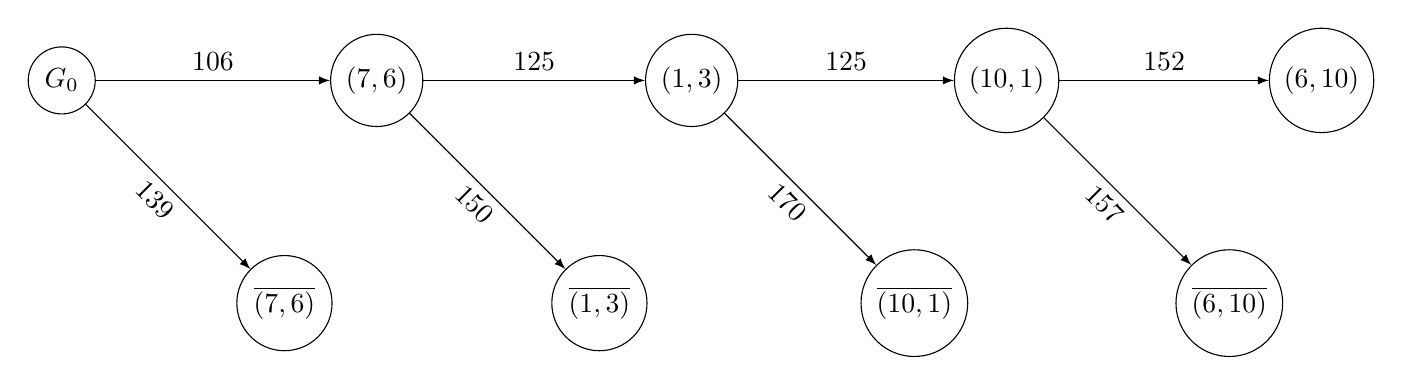
\begin{tikzpicture}[
        grow=east, % Дерево растет слева направо
        level 1/.style = {level distance=4cm}, % Расстояние между уровнями
        edge from parent/.style = {draw, -latex},
        kant/.style={text width=2cm, text centered, sloped},
        cell/.style={circle, draw, align=center}, % Стиль узлов
    ]

    \node[cell] {$G_0$}
    child[grow=east] {node[cell] {$(7, 6)$}
            child[grow=east] {node[cell] {$(1, 3)$}
                    child[grow=east] {node[cell] {$(10, 1)$}
                            child[grow=east] {node[cell] {$(6, 10)$} edge from parent node[kant, above] {152}}
                            child[grow=south east] {node[cell] {$\overline{(6, 10)}$} edge from parent node[kant, below] {157}}
                            edge from parent node[kant, above] {125}}
                    child[grow=south east] {node[cell] {$\overline{(10, 1)}$} edge from parent node[kant, below] {170}}
                    edge from parent node[kant, above] {125}}
            child[grow=south east] {node[cell] {$\overline{(1, 3)}$} edge from parent node[kant, below] {150}}
            edge from parent node[kant, above] {106}}
    child[grow=south east] {node[cell] {$\overline{(7, 6)}$} edge from parent node[kant, below] {139}};
\end{tikzpicture}

Найдём претендентов на ветвление:

\[
    \begin{array}{|>{\columncolor{lightgray}}c|c|c|c|c|c|c|c|c|c|c|c|c|c|}
        \hline
        S      & (2, 7) & (3, 2) & (3, 4) & (4, 7) & (5, 8) & (5, 9) & (8, 4) & (8, 5) & (9, 8) \\
        \hline
        d_i    & 1      & 0      & 0      & 1      & 0      & 0      & 0      & 0      & 20     \\
        \hline
        d_j    & 0      & 1      & 0      & 0      & 0      & 14     & 0      & 8      & 0      \\
        \hline
        Q_{ij} & 1      & 1      & 0      & 1      & 0      & 14     & 0      & 8      & 20     \\
        \hline
    \end{array}
\]

$\max Q_{ij} = Q_{9, 8} = 20$. Ветвление производим по элементу $(9, 8)$.

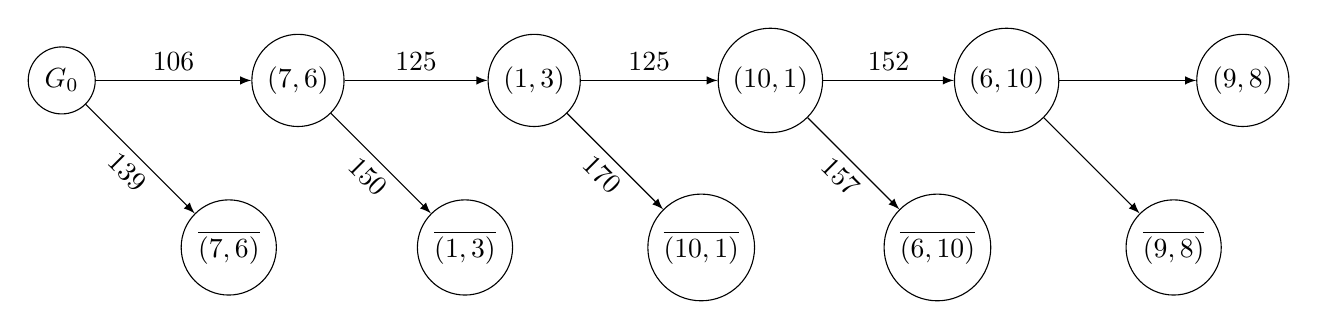
\begin{tikzpicture}[
        grow=east, % Дерево растет слева направо
        level 1/.style = {level distance=3cm}, % Расстояние между уровнями
        edge from parent/.style = {draw, -latex},
        kant/.style={text width=2cm, text centered, sloped},
        cell/.style={circle, draw, align=center}, % Стиль узлов
    ]

    \node[cell] {$G_0$}
    child[grow=east] {node[cell] {$(7, 6)$}
            child[grow=east] {node[cell] {$(1, 3)$}
                    child[grow=east] {node[cell] {$(10, 1)$}
                            child[grow=east] {node[cell] {$(6, 10)$}
                                    child[grow=east] {node[cell] {$(9, 8)$}}
                                    child[grow=south east] {node[cell] {$\overline{(9, 8)}$}}
                                    edge from parent node[kant, above] {152}}
                            child[grow=south east] {node[cell] {$\overline{(6, 10)}$} edge from parent node[kant, below] {157}}
                            edge from parent node[kant, above] {125}}
                    child[grow=south east] {node[cell] {$\overline{(10, 1)}$} edge from parent node[kant, below] {170}}
                    edge from parent node[kant, above] {125}}
            child[grow=south east] {node[cell] {$\overline{(1, 3)}$} edge from parent node[kant, below] {150}}
            edge from parent node[kant, above] {106}}
    child[grow=south east] {node[cell] {$\overline{(7, 6)}$} edge from parent node[kant, below] {139}};
\end{tikzpicture}

Находим оценку множества $\overline{(9, 8)}$: $w(\overline{(9, 8)}) = w((6, 10)) + Q_{9, 8} = 152 + 20 = 172$.

Находим оценку множества $(9, 8)$. Для этого нужно вычеркнуть из таблицы строку 9 и столбец 8, а также исключить циклы: поставить $\infty$ в ячейку $(8, 9)$, чтобы не возникло цикла $9 \to 8 \to 9$. И редуцировать эту таблицу.

\[
    \begin{array}{|>{\columncolor{lightgray}}c|c|c|c|c|c|>{\columncolor{LightBlue}}c|}
        \hline \rowcolor{lightgray}
        \text{Город} & 2      & 4      & 5      & 7      & 9      & \text{min}             \\
        \hline
        2            & \infty & 1      & 16     & 0      & 14     & 0                      \\
        \hline
        3            & 0      & 0      & 8      & \infty & 54     & 0                      \\
        \hline
        4            & 1      & \infty & 41     & 0      & 33     & 0                      \\
        \hline
        5            & 1      & 57     & \infty & 44     & 0      & 0                      \\
        \hline
        8            & 5      & 0      & 0      & 2      & \infty & 0                      \\
        \hline \rowcolor{LightBlue}
        \text{min}   & 0      & 0      & 0      & 0      & 0      & \cellcolor{Chocolate}0 \\
        \hline
    \end{array}
\]

$h = 0$. Это значит, что $w((9, 8)) = w((6, 10)) + h = 152 + 0 = 152$.

$w(\overline{(9, 8)}) = 172$, $w((9, 8)) = 152$. Выбираем ветвь с меньшей оценкой, то есть $(9, 8)$.

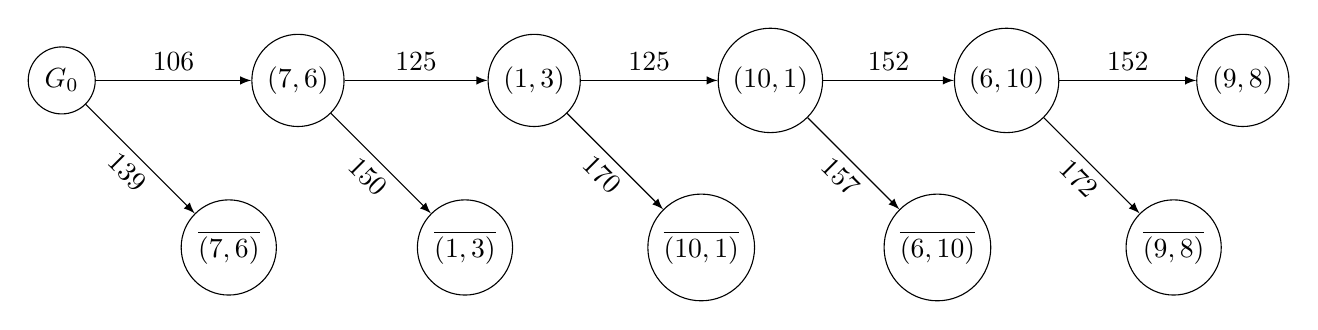
\begin{tikzpicture}[
        grow=east, % Дерево растет слева направо
        level 1/.style = {level distance=3cm}, % Расстояние между уровнями
        edge from parent/.style = {draw, -latex},
        kant/.style={text width=2cm, text centered, sloped},
        cell/.style={circle, draw, align=center}, % Стиль узлов
    ]

    \node[cell] {$G_0$}
    child[grow=east] {node[cell] {$(7, 6)$}
            child[grow=east] {node[cell] {$(1, 3)$}
                    child[grow=east] {node[cell] {$(10, 1)$}
                            child[grow=east] {node[cell] {$(6, 10)$}
                                    child[grow=east] {node[cell] {$(9, 8)$} edge from parent node[kant, above] {152}}
                                    child[grow=south east] {node[cell] {$\overline{(9, 8)}$} edge from parent node[kant, below] {172}}
                                    edge from parent node[kant, above] {152}}
                            child[grow=south east] {node[cell] {$\overline{(6, 10)}$} edge from parent node[kant, below] {157}}
                            edge from parent node[kant, above] {125}}
                    child[grow=south east] {node[cell] {$\overline{(10, 1)}$} edge from parent node[kant, below] {170}}
                    edge from parent node[kant, above] {125}}
            child[grow=south east] {node[cell] {$\overline{(1, 3)}$} edge from parent node[kant, below] {150}}
            edge from parent node[kant, above] {106}}
    child[grow=south east] {node[cell] {$\overline{(7, 6)}$} edge from parent node[kant, below] {139}};
\end{tikzpicture}

Найдём претендентов на ветвление:

\[
    \begin{array}{|>{\columncolor{lightgray}}c|c|c|c|c|c|c|c|c|c|c|c|c|c|}
        \hline
        S      & (2, 7) & (3, 2) & (3, 4) & (4, 7) & (5, 9) & (8, 4) & (8, 5) \\
        \hline
        d_i    & 1      & 0      & 0      & 1      & 1      & 0      & 0      \\
        \hline
        d_j    & 0      & 1      & 0      & 0      & 14     & 0      & 8      \\
        \hline
        Q_{ij} & 1      & 1      & 0      & 1      & 15     & 0      & 8      \\
        \hline
    \end{array}
\]

$\max Q_{ij} = Q_{5, 9} = 15$. Ветвление производим по элементу $(5, 9)$.

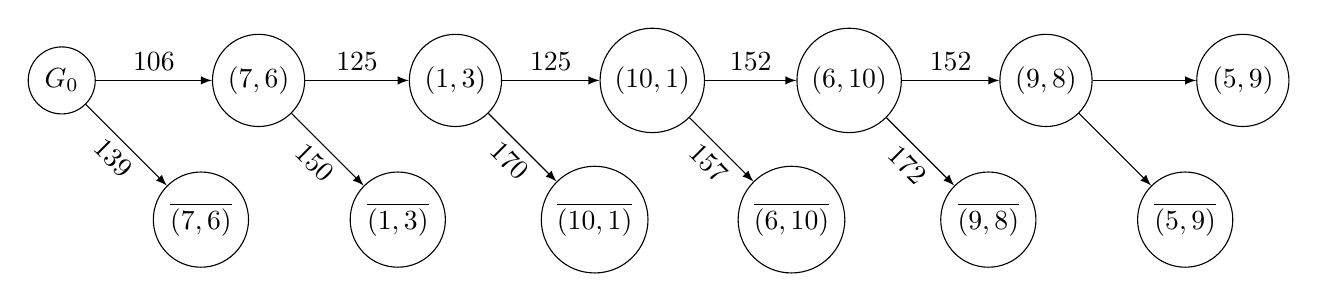
\begin{tikzpicture}[
        grow=east, % Дерево растет слева направо
        level 1/.style = {level distance=2.5cm}, % Расстояние между уровнями
        edge from parent/.style = {draw, -latex},
        kant/.style={text width=2cm, text centered, sloped},
        cell/.style={circle, draw, align=center}, % Стиль узлов
    ]

    \node[cell] {$G_0$}
    child[grow=east] {node[cell] {$(7, 6)$}
            child[grow=east] {node[cell] {$(1, 3)$}
                    child[grow=east] {node[cell] {$(10, 1)$}
                            child[grow=east] {node[cell] {$(6, 10)$}
                                    child[grow=east] {node[cell] {$(9, 8)$}
                                            child[grow=east] {node[cell] {$(5, 9)$}}
                                            child[grow=south east] {node[cell] {$\overline{(5, 9)}$}}
                                            edge from parent node[kant, above] {152}}
                                    child[grow=south east] {node[cell] {$\overline{(9, 8)}$} edge from parent node[kant, below] {172}}
                                    edge from parent node[kant, above] {152}}
                            child[grow=south east] {node[cell] {$\overline{(6, 10)}$} edge from parent node[kant, below] {157}}
                            edge from parent node[kant, above] {125}}
                    child[grow=south east] {node[cell] {$\overline{(10, 1)}$} edge from parent node[kant, below] {170}}
                    edge from parent node[kant, above] {125}}
            child[grow=south east] {node[cell] {$\overline{(1, 3)}$} edge from parent node[kant, below] {150}}
            edge from parent node[kant, above] {106}}
    child[grow=south east] {node[cell] {$\overline{(7, 6)}$} edge from parent node[kant, below] {139}};
\end{tikzpicture}

Находим оценку множества $\overline{(5, 9)}$: $w(\overline{(5, 9)}) = w((9, 8)) + Q_{5, 9} = 152 + 15 = 167$.

Находим оценку множества $(5, 9)$. Для этого нужно вычеркнуть из таблицы строку 5 и столбец 9, а также исключить циклы: поставить $\infty$ в ячейку $(8, 5)$, чтобы не возникло цикла $5 \to 9 \to 8 \to 5$. И редуцировать эту таблицу.

\[
    \begin{array}{|>{\columncolor{lightgray}}c|c|c|c|c|>{\columncolor{LightBlue}}c|}
        \hline \rowcolor{lightgray}
        \text{Город} & 2      & 4      & 5      & 7      & \text{min}             \\
        \hline
        2            & \infty & 1      & 8      & 0      & 0                      \\
        \hline
        3            & 0      & 0      & 0      & \infty & 0                      \\
        \hline
        4            & 1      & \infty & 33     & 0      & 0                      \\
        \hline
        8            & 5      & 0      & \infty & 2      & 0                      \\
        \hline \rowcolor{LightBlue}
        \text{min}   & 0      & 0      & 8      & 0      & \cellcolor{Chocolate}8 \\
        \hline
    \end{array}
\]

$h = 8$. Это значит, что $w((5, 9)) = w((9, 8)) + h = 152 + 8 = 160$.

$w(\overline{(5, 9)}) = 167$, $w((5, 9)) = 160$. Выбираем ветвь с меньшей оценкой, то есть $(5, 9)$.

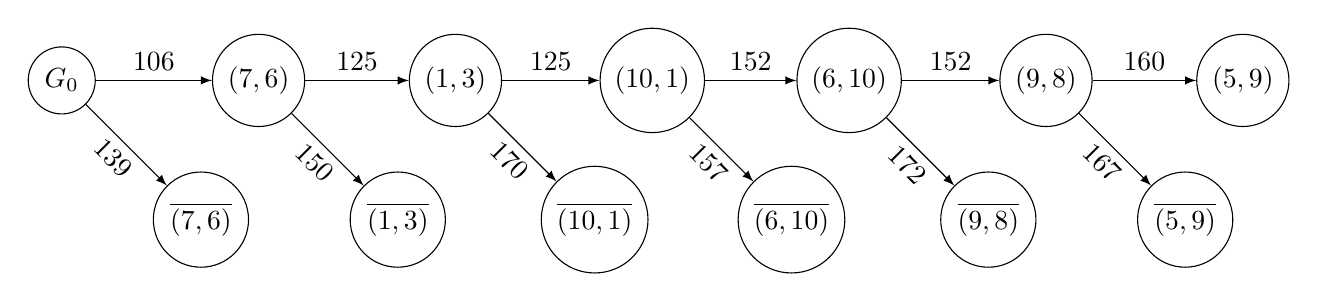
\begin{tikzpicture}[
        grow=east, % Дерево растет слева направо
        level 1/.style = {level distance=2.5cm}, % Расстояние между уровнями
        edge from parent/.style = {draw, -latex},
        kant/.style={text width=2cm, text centered, sloped},
        cell/.style={circle, draw, align=center}, % Стиль узлов
    ]

    \node[cell] {$G_0$}
    child[grow=east] {node[cell] {$(7, 6)$}
            child[grow=east] {node[cell] {$(1, 3)$}
                    child[grow=east] {node[cell] {$(10, 1)$}
                            child[grow=east] {node[cell] {$(6, 10)$}
                                    child[grow=east] {node[cell] {$(9, 8)$}
                                            child[grow=east] {node[cell] {$(5, 9)$} edge from parent node[kant, above] {160}}
                                            child[grow=south east] {node[cell] {$\overline{(5, 9)}$} edge from parent node[kant, below] {167}}
                                            edge from parent node[kant, above] {152}}
                                    child[grow=south east] {node[cell] {$\overline{(9, 8)}$} edge from parent node[kant, below] {172}}
                                    edge from parent node[kant, above] {152}}
                            child[grow=south east] {node[cell] {$\overline{(6, 10)}$} edge from parent node[kant, below] {157}}
                            edge from parent node[kant, above] {125}}
                    child[grow=south east] {node[cell] {$\overline{(10, 1)}$} edge from parent node[kant, below] {170}}
                    edge from parent node[kant, above] {125}}
            child[grow=south east] {node[cell] {$\overline{(1, 3)}$} edge from parent node[kant, below] {150}}
            edge from parent node[kant, above] {106}}
    child[grow=south east] {node[cell] {$\overline{(7, 6)}$} edge from parent node[kant, below] {139}};
\end{tikzpicture}

Найдём претендентов на ветвление:

\[
    \begin{array}{|>{\columncolor{lightgray}}c|c|c|c|c|c|c|c|c|c|c|c|c|c|}
        \hline
        S      & (2, 7) & (3, 2) & (3, 4) & (3, 5) & (4, 7) & (8, 4) \\
        \hline
        d_i    & 1      & 0      & 0      & 0      & 1      & 0      \\
        \hline
        d_j    & 0      & 1      & 0      & 8      & 0      & 0      \\
        \hline
        Q_{ij} & 1      & 1      & 0      & 8      & 1      & 0      \\
        \hline
    \end{array}
\]

$\max Q_{ij} = Q_{3, 5} = 8$. Ветвление производим по элементу $(3, 5)$.

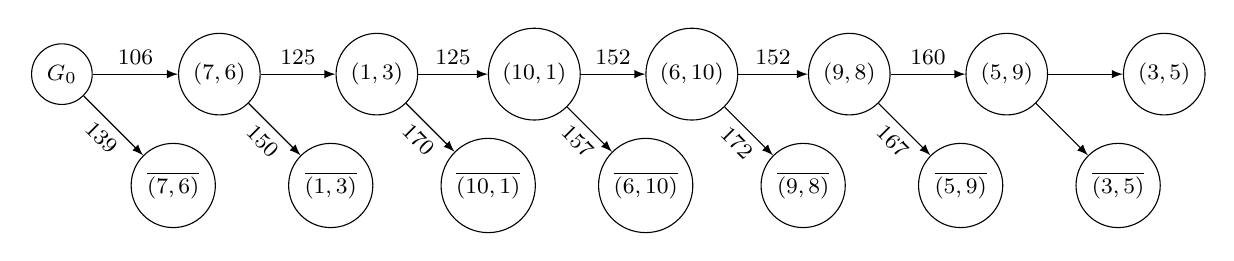
\begin{tikzpicture}[
        grow=east, % Дерево растет слева направо
        level 1/.style = {level distance=2cm}, % Расстояние между уровнями
        edge from parent/.style = {draw, -latex},
        kant/.style={text width=2cm, text centered, sloped, font=\footnotesize},
        cell/.style={circle, draw, align=center, font=\footnotesize}, % Стиль узлов
    ]

    \node[cell] {$G_0$}
    child[grow=east] {node[cell] {$(7, 6)$}
            child[grow=east] {node[cell] {$(1, 3)$}
                    child[grow=east] {node[cell] {$(10, 1)$}
                            child[grow=east] {node[cell] {$(6, 10)$}
                                    child[grow=east] {node[cell] {$(9, 8)$}
                                            child[grow=east] {node[cell] {$(5, 9)$}
                                                    child[grow=east] {node[cell] {$(3, 5)$}}
                                                    child[grow=south east] {node[cell] {$\overline{(3, 5)}$}}
                                                    edge from parent node[kant, above] {160}}
                                            child[grow=south east] {node[cell] {$\overline{(5, 9)}$} edge from parent node[kant, below] {167}}
                                            edge from parent node[kant, above] {152}}
                                    child[grow=south east] {node[cell] {$\overline{(9, 8)}$} edge from parent node[kant, below] {172}}
                                    edge from parent node[kant, above] {152}}
                            child[grow=south east] {node[cell] {$\overline{(6, 10)}$} edge from parent node[kant, below] {157}}
                            edge from parent node[kant, above] {125}}
                    child[grow=south east] {node[cell] {$\overline{(10, 1)}$} edge from parent node[kant, below] {170}}
                    edge from parent node[kant, above] {125}}
            child[grow=south east] {node[cell] {$\overline{(1, 3)}$} edge from parent node[kant, below] {150}}
            edge from parent node[kant, above] {106}}
    child[grow=south east] {node[cell] {$\overline{(7, 6)}$} edge from parent node[kant, below] {139}};
\end{tikzpicture}

Находим оценку множества $\overline{(3, 5)}$: $w(\overline{(3, 5)}) = w((5, 9)) + Q_{3, 5} = 160 + 8 = 168$.

Находим оценку множества $(3, 5)$. Для этого нужно вычеркнуть из таблицы строку 3 и столбец 5, циклы в данном случае уже исключены.

\[
    \begin{array}{|>{\columncolor{lightgray}}c|c|c|c|>{\columncolor{LightBlue}}c|}
        \hline \rowcolor{lightgray}
        \text{Город} & 2      & 4      & 7 & \text{min}             \\
        \hline
        2            & \infty & 1      & 0 & 0                      \\
        \hline
        4            & 0      & \infty & 0 & 0                      \\
        \hline
        8            & 4      & 0      & 2 & 0                      \\
        \hline \rowcolor{LightBlue}
        \text{min}   & 1      & 0      & 0 & \cellcolor{Chocolate}1 \\
        \hline
    \end{array}
\]

$h = 1$. Это значит, что $w((3, 5)) = w((5, 9)) + h = 160 + 1 = 161$.

$w(\overline{(3, 5)}) = 168$, $w((3, 5)) = 161$. Выбираем ветвь с меньшей оценкой, то есть $(3, 5)$.

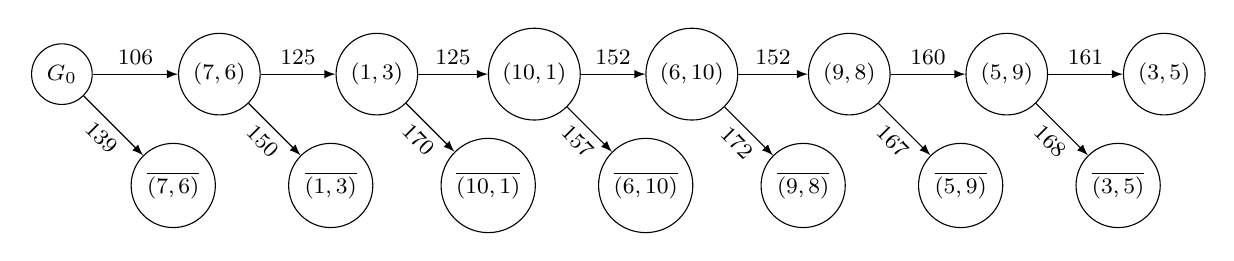
\begin{tikzpicture}[
        grow=east, % Дерево растет слева направо
        level 1/.style = {level distance=2cm}, % Расстояние между уровнями
        edge from parent/.style = {draw, -latex},
        kant/.style={text width=2cm, text centered, sloped, font=\footnotesize},
        cell/.style={circle, draw, align=center, font=\footnotesize}, % Стиль узлов
    ]

    \node[cell] {$G_0$}
    child[grow=east] {node[cell] {$(7, 6)$}
            child[grow=east] {node[cell] {$(1, 3)$}
                    child[grow=east] {node[cell] {$(10, 1)$}
                            child[grow=east] {node[cell] {$(6, 10)$}
                                    child[grow=east] {node[cell] {$(9, 8)$}
                                            child[grow=east] {node[cell] {$(5, 9)$}
                                                    child[grow=east] {node[cell] {$(3, 5)$} edge from parent node[kant, above] {161}}
                                                    child[grow=south east] {node[cell] {$\overline{(3, 5)}$} edge from parent node[kant, below] {168}}
                                                    edge from parent node[kant, above] {160}}
                                            child[grow=south east] {node[cell] {$\overline{(5, 9)}$} edge from parent node[kant, below] {167}}
                                            edge from parent node[kant, above] {152}}
                                    child[grow=south east] {node[cell] {$\overline{(9, 8)}$} edge from parent node[kant, below] {172}}
                                    edge from parent node[kant, above] {152}}
                            child[grow=south east] {node[cell] {$\overline{(6, 10)}$} edge from parent node[kant, below] {157}}
                            edge from parent node[kant, above] {125}}
                    child[grow=south east] {node[cell] {$\overline{(10, 1)}$} edge from parent node[kant, below] {170}}
                    edge from parent node[kant, above] {125}}
            child[grow=south east] {node[cell] {$\overline{(1, 3)}$} edge from parent node[kant, below] {150}}
            edge from parent node[kant, above] {106}}
    child[grow=south east] {node[cell] {$\overline{(7, 6)}$} edge from parent node[kant, below] {139}};
\end{tikzpicture}

Найдём претендентов на ветвление:

\[
    \begin{array}{|>{\columncolor{lightgray}}c|c|c|c|c|c|c|c|c|c|c|c|c|c|}
        \hline
        S      & (2, 7) & (4, 2) & (4, 7) & (8, 4) \\
        \hline
        d_i    & 1      & 0      & 0      & 2      \\
        \hline
        d_j    & 0      & 4      & 0      & 1      \\
        \hline
        Q_{ij} & 1      & 4      & 0      & 3      \\
        \hline
    \end{array}
\]

$\max Q_{ij} = Q_{4, 2} = 4$. Ветвление производим по элементу $(4, 2)$.

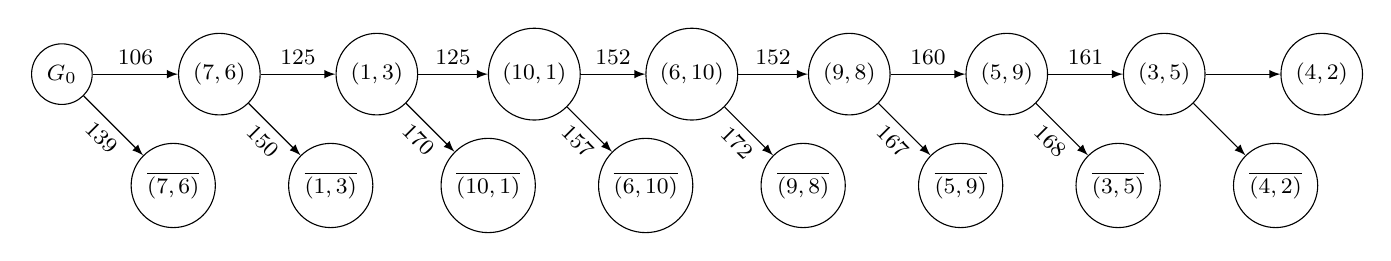
\begin{tikzpicture}[
        grow=east, % Дерево растет слева направо
        level 1/.style = {level distance=2cm}, % Расстояние между уровнями
        edge from parent/.style = {draw, -latex},
        kant/.style={text width=2cm, text centered, sloped, font=\footnotesize},
        cell/.style={circle, draw, align=center, font=\footnotesize}, % Стиль узлов
    ]

    \node[cell] {$G_0$}
    child[grow=east] {node[cell] {$(7, 6)$}
            child[grow=east] {node[cell] {$(1, 3)$}
                    child[grow=east] {node[cell] {$(10, 1)$}
                            child[grow=east] {node[cell] {$(6, 10)$}
                                    child[grow=east] {node[cell] {$(9, 8)$}
                                            child[grow=east] {node[cell] {$(5, 9)$}
                                                    child[grow=east] {node[cell] {$(3, 5)$}
                                                            child[grow=east] {node[cell] {$(4, 2)$}}
                                                            child[grow=south east] {node[cell] {$\overline{(4, 2)}$}}
                                                            edge from parent node[kant, above] {161}}
                                                    child[grow=south east] {node[cell] {$\overline{(3, 5)}$} edge from parent node[kant, below] {168}}
                                                    edge from parent node[kant, above] {160}}
                                            child[grow=south east] {node[cell] {$\overline{(5, 9)}$} edge from parent node[kant, below] {167}}
                                            edge from parent node[kant, above] {152}}
                                    child[grow=south east] {node[cell] {$\overline{(9, 8)}$} edge from parent node[kant, below] {172}}
                                    edge from parent node[kant, above] {152}}
                            child[grow=south east] {node[cell] {$\overline{(6, 10)}$} edge from parent node[kant, below] {157}}
                            edge from parent node[kant, above] {125}}
                    child[grow=south east] {node[cell] {$\overline{(10, 1)}$} edge from parent node[kant, below] {170}}
                    edge from parent node[kant, above] {125}}
            child[grow=south east] {node[cell] {$\overline{(1, 3)}$} edge from parent node[kant, below] {150}}
            edge from parent node[kant, above] {106}}
    child[grow=south east] {node[cell] {$\overline{(7, 6)}$} edge from parent node[kant, below] {139}};
\end{tikzpicture}

Находим оценку множества $\overline{(4, 2)}$: $w(\overline{(4, 2)}) = w((3, 5)) + Q_{4, 2} = 161 + 4 = 165$.

Находим оценку множества $(4, 2)$. Для этого нужно вычеркнуть из таблицы строку 4 и столбец 2. А также исключить циклы: поставить $\infty$ в ячейку $(2, 4)$, чтобы не возникло цикла $4 \to 2 \to 4$. И редуцировать эту таблицу.

\[
    \begin{array}{|>{\columncolor{lightgray}}c|c|c|>{\columncolor{LightBlue}}c|}
        \hline \rowcolor{lightgray}
        \text{Город} & 4      & 7 & \text{min}             \\
        \hline
        2            & \infty & 0 & 0                      \\
        \hline
        8            & 0      & 2 & 0                      \\
        \hline \rowcolor{LightBlue}
        \text{min}   & 0      & 0 & \cellcolor{Chocolate}0 \\
        \hline
    \end{array}
\]

$h = 0$. Это значит, что $w((4, 2)) = w((3, 5)) + h = 161 + 0 = 161$.

$w(\overline{(4, 2)}) = 165$, $w((4, 2)) = 161$. Выбираем ветвь с меньшей оценкой, то есть $(4, 2)$.

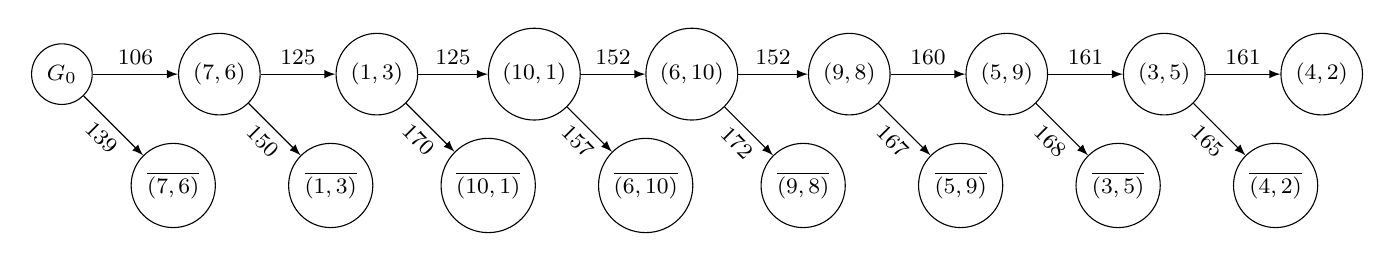
\begin{tikzpicture}[
        grow=east, % Дерево растет слева направо
        level 1/.style = {level distance=2cm}, % Расстояние между уровнями
        edge from parent/.style = {draw, -latex},
        kant/.style={text width=2cm, text centered, sloped, font=\footnotesize},
        cell/.style={circle, draw, align=center, font=\footnotesize}, % Стиль узлов
    ]

    \node[cell] {$G_0$}
    child[grow=east] {node[cell] {$(7, 6)$}
            child[grow=east] {node[cell] {$(1, 3)$}
                    child[grow=east] {node[cell] {$(10, 1)$}
                            child[grow=east] {node[cell] {$(6, 10)$}
                                    child[grow=east] {node[cell] {$(9, 8)$}
                                            child[grow=east] {node[cell] {$(5, 9)$}
                                                    child[grow=east] {node[cell] {$(3, 5)$}
                                                            child[grow=east] {node[cell] {$(4, 2)$} edge from parent node[kant, above] {161}}
                                                            child[grow=south east] {node[cell] {$\overline{(4, 2)}$} edge from parent node[kant, below] {165}}
                                                            edge from parent node[kant, above] {161}}
                                                    child[grow=south east] {node[cell] {$\overline{(3, 5)}$} edge from parent node[kant, below] {168}}
                                                    edge from parent node[kant, above] {160}}
                                            child[grow=south east] {node[cell] {$\overline{(5, 9)}$} edge from parent node[kant, below] {167}}
                                            edge from parent node[kant, above] {152}}
                                    child[grow=south east] {node[cell] {$\overline{(9, 8)}$} edge from parent node[kant, below] {172}}
                                    edge from parent node[kant, above] {152}}
                            child[grow=south east] {node[cell] {$\overline{(6, 10)}$} edge from parent node[kant, below] {157}}
                            edge from parent node[kant, above] {125}}
                    child[grow=south east] {node[cell] {$\overline{(10, 1)}$} edge from parent node[kant, below] {170}}
                    edge from parent node[kant, above] {125}}
            child[grow=south east] {node[cell] {$\overline{(1, 3)}$} edge from parent node[kant, below] {150}}
            edge from parent node[kant, above] {106}}
    child[grow=south east] {node[cell] {$\overline{(7, 6)}$} edge from parent node[kant, below] {139}};
\end{tikzpicture}

Осталась матрица $2 \times 2$. Очевидно, что она уже не нуждается в ветвлении, и нужно брать рёбра $(2, 7)$ и $(8, 4)$. Для обоих множества $w((2, 7)) = w((8, 4)) = 0$.

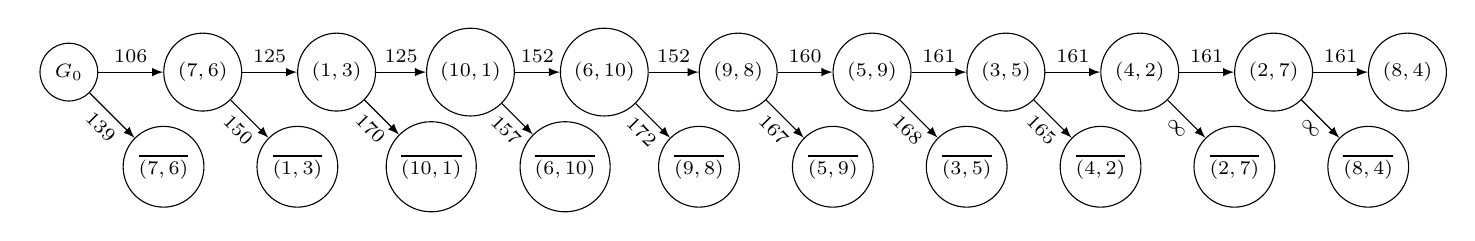
\begin{tikzpicture}[
        grow=east, % Дерево растет слева направо
        level 1/.style = {level distance=1.70cm}, % Расстояние между уровнями
        edge from parent/.style = {draw, -latex},
        kant/.style={text width=2cm, text centered, sloped, font=\scriptsize},
        cell/.style={circle, draw, align=center, font=\scriptsize}, % Стиль узлов
    ]

    \node[cell] {$G_0$}
    child[grow=east] {node[cell] {$(7, 6)$}
            child[grow=east] {node[cell] {$(1, 3)$}
                    child[grow=east] {node[cell] {$(10, 1)$}
                            child[grow=east] {node[cell] {$(6, 10)$}
                                    child[grow=east] {node[cell] {$(9, 8)$}
                                            child[grow=east] {node[cell] {$(5, 9)$}
                                                    child[grow=east] {node[cell] {$(3, 5)$}
                                                            child[grow=east] {node[cell] {$(4, 2)$}
                                                                    child[grow=east] {node[cell] {$(2, 7)$}
                                                                            child[grow=east] {node[cell] {$(8, 4)$} edge from parent node[kant, above] {161}}
                                                                            child[grow=south east] {node[cell] {$\overline{(8, 4)}$} edge from parent node[kant, below] {$\infty$}}
                                                                            edge from parent node[kant, above] {161}}
                                                                    child[grow=south east] {node[cell] {$\overline{(2, 7)}$} edge from parent node[kant, below] {$\infty$}}
                                                                    edge from parent node[kant, above] {161}}
                                                            child[grow=south east] {node[cell] {$\overline{(4, 2)}$} edge from parent node[kant, below] {165}}
                                                            edge from parent node[kant, above] {161}}
                                                    child[grow=south east] {node[cell] {$\overline{(3, 5)}$} edge from parent node[kant, below] {168}}
                                                    edge from parent node[kant, above] {160}}
                                            child[grow=south east] {node[cell] {$\overline{(5, 9)}$} edge from parent node[kant, below] {167}}
                                            edge from parent node[kant, above] {152}}
                                    child[grow=south east] {node[cell] {$\overline{(9, 8)}$} edge from parent node[kant, below] {172}}
                                    edge from parent node[kant, above] {152}}
                            child[grow=south east] {node[cell] {$\overline{(6, 10)}$} edge from parent node[kant, below] {157}}
                            edge from parent node[kant, above] {125}}
                    child[grow=south east] {node[cell] {$\overline{(10, 1)}$} edge from parent node[kant, below] {170}}
                    edge from parent node[kant, above] {125}}
            child[grow=south east] {node[cell] {$\overline{(1, 3)}$} edge from parent node[kant, below] {150}}
            edge from parent node[kant, above] {106}}
    child[grow=south east] {node[cell] {$\overline{(7, 6)}$} edge from parent node[kant, below] {139}};
\end{tikzpicture}

\textbf{Критерий оптимальности:} Если оценка последнего множества не больше оценок всех тупиковых ветвей, то маршрут, описанный деревом ветвей, является оптимальным.

Оценки тупиковых ветвей, которые больше, чем оценка последнего множества: $w(\overline{(7, 6)}) = 139, w(\overline{(1, 3)}) = 150, w(\overline{(6, 10)}) = 157$. Оценка последнего множества: $w((8, 4)) = 161$.

Процесс ветвления должен быть продолжен для этих тупиковых ветвей и может быть остановлен, когда оценка последнего множества окажется не больше оценок всех тупиковых ветвей.

Начнём ветвление для $\overline{(7, 6)}$. Для этого в таблицу для $G_0$ поставим $\infty$ в ячейку $(7, 6)$:

\[
    \begin{array}{|>{\columncolor{lightgray}}c|c|c|c|c|c|c|c|c|c|c|>{\columncolor{LightBlue}}c|}
        \hline \rowcolor{lightgray}
        \text{Город} & 1      & 2      & 3      & 4      & 5      & 6      & 7      & 8      & 9      & 10     & \text{min}            \\
        \hline
        1            & \infty & 62     & 0      & 57     & 42     & 6      & 68     & 72     & 46     & 60     &                       \\
        \hline
        2            & 86     & \infty & 22     & 1      & 16     & 51     & 0      & 86     & 14     & 36     &                       \\
        \hline
        3            & 0      & 46     & \infty & 19     & 27     & 74     & 56     & 20     & 73     & 47     &                       \\
        \hline
        4            & 76     & 28     & 27     & \infty & 41     & 65     & 0      & 47     & 33     & 32     &                       \\
        \hline
        5            & 55     & 28     & 48     & 57     & \infty & 94     & 44     & 0      & 0      & 66     &                       \\
        \hline
        6            & 37     & 0      & 2      & 87     & 54     & \infty & 7      & 88     & 37     & 0      &                       \\
        \hline
        7            & 76     & 68     & 52     & 63     & 32     & \infty & \infty & 27     & 56     & 73     &                       \\
        \hline
        8            & 34     & 32     & 2      & 0      & 0      & 52     & 2      & \infty & 77     & 61     &                       \\
        \hline
        9            & 4      & 60     & 30     & 20     & 56     & 48     & 86     & 0      & \infty & 34     &                       \\
        \hline
        10           & 0      & 41     & 63     & 72     & 43     & 25     & 70     & 65     & 53     & \infty &                       \\
        \hline \rowcolor{LightBlue}
        \text{min}   &        &        &        &        &        &        &        &        &        &        & \cellcolor{Chocolate} \\
        \hline
    \end{array}
\]

И потом проведём процесс редуцирования:

\[
    \begin{array}{|>{\columncolor{lightgray}}c|c|c|c|c|c|c|c|c|c|c|>{\columncolor{LightBlue}}c|}
        \hline \rowcolor{lightgray}
        \text{Город} & 1      & 2      & 3      & 4      & 5      & 6      & 7      & 8      & 9      & 10     & \text{min}              \\
        \hline
        1            & \infty & 62     & 0      & 57     & 42     & 0      & 68     & 72     & 46     & 60     & 0                       \\
        \hline
        2            & 86     & \infty & 22     & 1      & 16     & 45     & 0      & 86     & 14     & 36     & 0                       \\
        \hline
        3            & 0      & 46     & \infty & 19     & 27     & 68     & 56     & 20     & 73     & 47     & 0                       \\
        \hline
        4            & 76     & 28     & 27     & \infty & 41     & 59     & 0      & 47     & 33     & 32     & 0                       \\
        \hline
        5            & 55     & 28     & 48     & 57     & \infty & 88     & 44     & 0      & 0      & 66     & 0                       \\
        \hline
        6            & 37     & 0      & 2      & 87     & 54     & \infty & 7      & 88     & 37     & 0      & 0                       \\
        \hline
        7            & 49     & 41     & 25     & 36     & 5      & \infty & \infty & 0      & 29     & 45     & 27                      \\
        \hline
        8            & 34     & 32     & 2      & 0      & 0      & 46     & 2      & \infty & 77     & 61     & 0                       \\
        \hline
        9            & 4      & 60     & 30     & 20     & 56     & 42     & 86     & 0      & \infty & 34     & 0                       \\
        \hline
        10           & 0      & 41     & 63     & 72     & 43     & 19     & 70     & 65     & 53     & \infty & 0                       \\
        \hline \rowcolor{LightBlue}
        \text{min}   & 0      & 0      & 0      & 0      & 0      & 6      & 0      & 0      & 0      & 0      & \cellcolor{Chocolate}33 \\
        \hline
    \end{array}
\]

Претенденты на ветвление:
{\small
\[
    \begin{array}{|>{\columncolor{lightgray}}c|c|c|c|c|c|c|c|c|c|c|c|c|c|c|}
        \hline
        S      & (1,3) & (1, 6) & (2, 7) & (3, 1) & (4, 7) & (5, 8) & (5, 9) & (6, 2) & (6, 10) & (7, 8) & (8, 4) & (8, 5) & (9, 8) & (10, 1) \\
        \hline
        d_i    & 0     & 0      & 1      & 19     & 27     & 0      & 0      & 0      & 0       & 5      & 0      & 0      & 4      & 19      \\
        \hline
        d_j    & 2     & 19     & 0      & 0      & 0      & 0      & 14     & 28     & 32      & 0      & 1      & 5      & 0      & 0       \\
        \hline
        Q_{ij} & 2     & 19     & 1      & 19     & 27     & 0      & 14     & 28     & 32      & 5      & 1      & 5      & 4      & 19      \\
        \hline
    \end{array}
\]
}

$\max Q_{ij} = Q_{6, 10} = 32$. Ветвление производим по элементу $(6, 10)$.

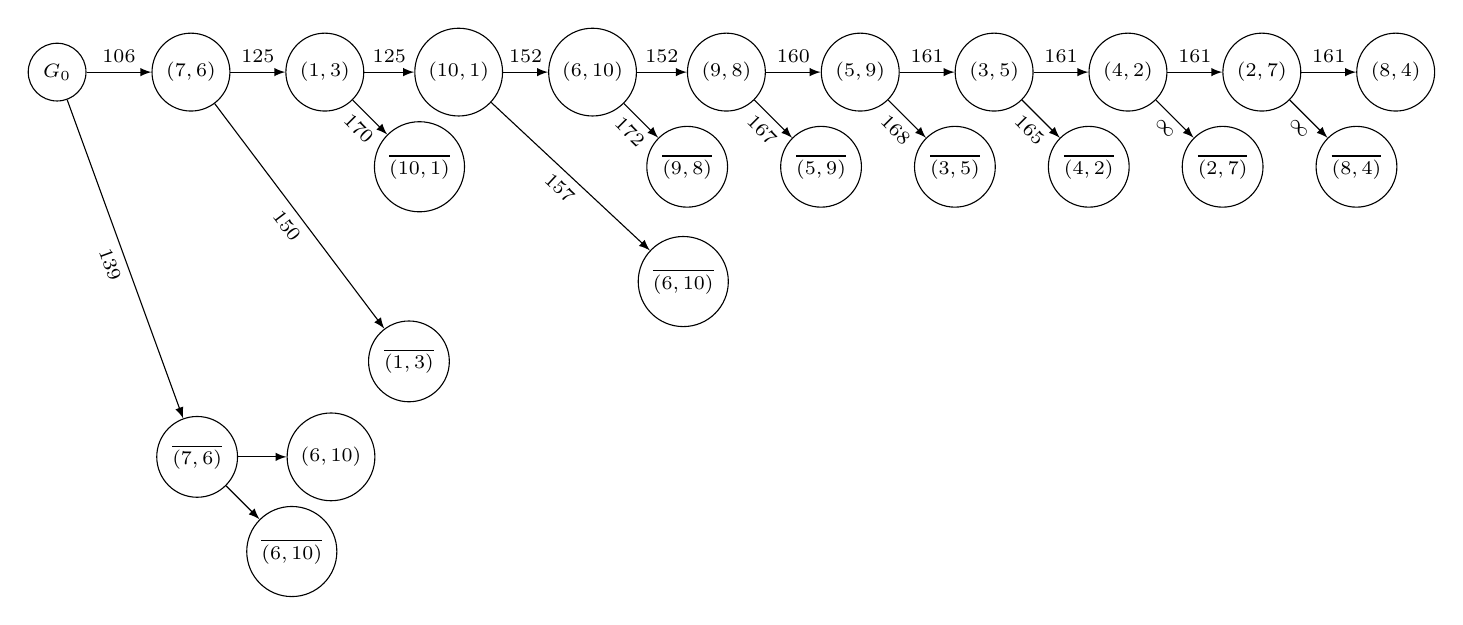
\begin{tikzpicture}[
        grow=east, % Дерево растет слева направо
        level 1/.style = {level distance=1.70cm}, % Расстояние между уровнями
        edge from parent/.style = {draw, -latex},
        kant/.style={text width=2cm, text centered, sloped, font=\scriptsize},
        cell/.style={circle, draw, align=center, font=\scriptsize}, % Стиль узлов
    ]

    \node[cell] {$G_0$}
    child[grow=east] {node[cell] {$(7, 6)$}
            child[grow=east] {node[cell] {$(1, 3)$}
                    child[grow=east] {node[cell] {$(10, 1)$}
                            child[grow=east] {node[cell] {$(6, 10)$}
                                    child[grow=east] {node[cell] {$(9, 8)$}
                                            child[grow=east] {node[cell] {$(5, 9)$}
                                                    child[grow=east] {node[cell] {$(3, 5)$}
                                                            child[grow=east] {node[cell] {$(4, 2)$}
                                                                    child[grow=east] {node[cell] {$(2, 7)$}
                                                                            child[grow=east] {node[cell] {$(8, 4)$} edge from parent node[kant, above] {161}}
                                                                            child[grow=south east] {node[cell] {$\overline{(8, 4)}$} edge from parent node[kant, below] {$\infty$}}
                                                                            edge from parent node[kant, above] {161}}
                                                                    child[grow=south east] {node[cell] {$\overline{(2, 7)}$} edge from parent node[kant, below] {$\infty$}}
                                                                    edge from parent node[kant, above] {161}}
                                                            child[grow=south east] {node[cell] {$\overline{(4, 2)}$} edge from parent node[kant, below] {165}}
                                                            edge from parent node[kant, above] {161}}
                                                    child[grow=south east] {node[cell] {$\overline{(3, 5)}$} edge from parent node[kant, below] {168}}
                                                    edge from parent node[kant, above] {160}}
                                            child[grow=south east] {node[cell] {$\overline{(5, 9)}$} edge from parent node[kant, below] {167}}
                                            edge from parent node[kant, above] {152}}
                                    child[grow=south east] {node[cell] {$\overline{(9, 8)}$} edge from parent node[kant, below] {172}}
                                    edge from parent node[kant, above] {152}}
                            child[grow=317, level distance=3.9cm] {node[cell] {$\overline{(6, 10)}$} edge from parent node[kant, below] {157}}
                            edge from parent node[kant, above] {125}}
                    child[grow=south east] {node[cell] {$\overline{(10, 1)}$} edge from parent node[kant, below] {170}}
                    edge from parent node[kant, above] {125}}
            child[grow=307, level distance=4.6cm] {node[cell] {$\overline{(1, 3)}$} edge from parent node[kant, below] {150}}
            edge from parent node[kant, above] {106}}
    child[grow=290, level distance=5.2cm] {node[cell] {$\overline{(7, 6)}$}
            child[grow=east, level distance=1.7cm] {node[cell] {$(6, 10)$}}
            child[grow=south east, level distance=1.7cm] {node[cell] {$\overline{(6, 10)}$}}
            edge from parent node[kant, below] {139}};
\end{tikzpicture}

Найдём оценку множества $\overline{(6, 10)}$: $w(\overline{(6, 10)}) = w(\overline{(7, 6)}) + Q_{6, 10} = 139 + 32 = 171$.

Находим оценку множества $(6, 10)$. Для этого нужно вычеркнуть из таблицы строку 6 и столбец 10. А также исключить циклы: поставить $\infty$ в ячейку $(10, 6)$, чтобы не возникло цикла $6 \to 10 \to 6$. И редуцировать эту таблицу.

\[
    \begin{array}{|>{\columncolor{lightgray}}c|c|c|c|c|c|c|c|c|c|>{\columncolor{LightBlue}}c|}
        \hline \rowcolor{lightgray}
        \text{Город} & 1      & 2      & 3      & 4      & 5      & 6      & 7      & 8      & 9      & \text{min}              \\
        \hline
        1            & \infty & 34     & 0      & 57     & 42     & 0      & 68     & 72     & 46     & 0                       \\
        \hline
        2            & 86     & \infty & 22     & 1      & 16     & 45     & 0      & 86     & 14     & 0                       \\
        \hline
        3            & 0      & 18     & \infty & 19     & 27     & 68     & 56     & 20     & 73     & 0                       \\
        \hline
        4            & 76     & 0      & 27     & \infty & 41     & 59     & 0      & 47     & 33     & 0                       \\
        \hline
        5            & 55     & 0      & 48     & 57     & \infty & 88     & 44     & 0      & 0      & 0                       \\
        \hline
        7            & 49     & 13     & 25     & 36     & 5      & \infty & \infty & 0      & 29     & 0                       \\
        \hline
        8            & 34     & 4      & 2      & 0      & 0      & 46     & 2      & \infty & 77     & 0                       \\
        \hline
        9            & 4      & 32     & 30     & 20     & 56     & 42     & 86     & 0      & \infty & 0                       \\
        \hline
        10           & 0      & 13     & 63     & 72     & 43     & \infty & 70     & 65     & 53     & 0                       \\
        \hline \rowcolor{LightBlue}
        \text{min}   & 0      & 28     & 0      & 0      & 0      & 0      & 0      & 0      & 0      & \cellcolor{Chocolate}28 \\
        \hline
    \end{array}
\]

$h = 28$. Это значит, что $w((6, 10)) = w(\overline{(7, 6)}) + h = 139 + 28 = 167$.

$w(\overline{(6, 10)}) = 171$, $w((6, 10)) = 167$. Заметим, что все они больше полученной нами ранее оценки $w((8, 4)) = 161$. Это значит, что мы можем остановить процесс ветвления для тупиковой ветви $\overline{(7, 6)}$.

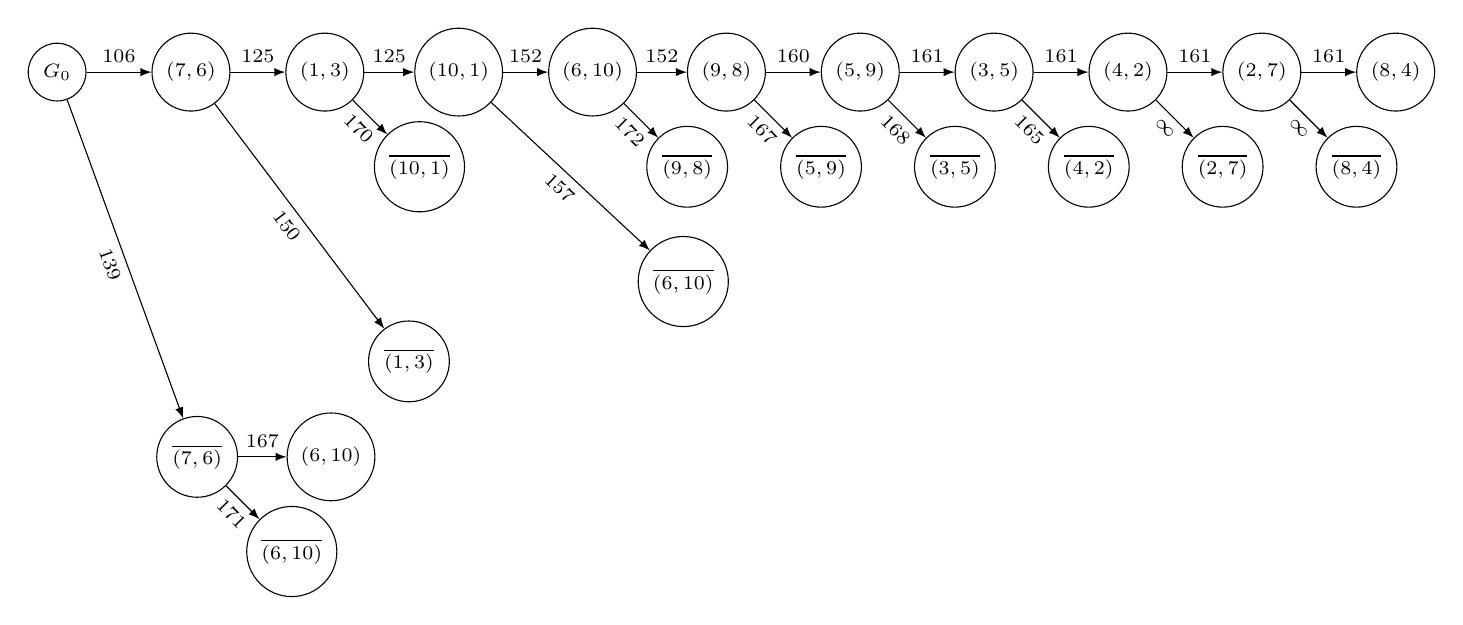
\begin{tikzpicture}[
        grow=east, % Дерево растет слева направо
        level 1/.style = {level distance=1.70cm}, % Расстояние между уровнями
        edge from parent/.style = {draw, -latex},
        kant/.style={text width=2cm, text centered, sloped, font=\scriptsize},
        cell/.style={circle, draw, align=center, font=\scriptsize}, % Стиль узлов
    ]

    \node[cell] {$G_0$}
    child[grow=east] {node[cell] {$(7, 6)$}
            child[grow=east] {node[cell] {$(1, 3)$}
                    child[grow=east] {node[cell] {$(10, 1)$}
                            child[grow=east] {node[cell] {$(6, 10)$}
                                    child[grow=east] {node[cell] {$(9, 8)$}
                                            child[grow=east] {node[cell] {$(5, 9)$}
                                                    child[grow=east] {node[cell] {$(3, 5)$}
                                                            child[grow=east] {node[cell] {$(4, 2)$}
                                                                    child[grow=east] {node[cell] {$(2, 7)$}
                                                                            child[grow=east] {node[cell] {$(8, 4)$} edge from parent node[kant, above] {161}}
                                                                            child[grow=south east] {node[cell] {$\overline{(8, 4)}$} edge from parent node[kant, below] {$\infty$}}
                                                                            edge from parent node[kant, above] {161}}
                                                                    child[grow=south east] {node[cell] {$\overline{(2, 7)}$} edge from parent node[kant, below] {$\infty$}}
                                                                    edge from parent node[kant, above] {161}}
                                                            child[grow=south east] {node[cell] {$\overline{(4, 2)}$} edge from parent node[kant, below] {165}}
                                                            edge from parent node[kant, above] {161}}
                                                    child[grow=south east] {node[cell] {$\overline{(3, 5)}$} edge from parent node[kant, below] {168}}
                                                    edge from parent node[kant, above] {160}}
                                            child[grow=south east] {node[cell] {$\overline{(5, 9)}$} edge from parent node[kant, below] {167}}
                                            edge from parent node[kant, above] {152}}
                                    child[grow=south east] {node[cell] {$\overline{(9, 8)}$} edge from parent node[kant, below] {172}}
                                    edge from parent node[kant, above] {152}}
                            child[grow=317, level distance=3.9cm] {node[cell] {$\overline{(6, 10)}$} edge from parent node[kant, below] {157}}
                            edge from parent node[kant, above] {125}}
                    child[grow=south east] {node[cell] {$\overline{(10, 1)}$} edge from parent node[kant, below] {170}}
                    edge from parent node[kant, above] {125}}
            child[grow=307, level distance=4.6cm] {node[cell] {$\overline{(1, 3)}$} edge from parent node[kant, below] {150}}
            edge from parent node[kant, above] {106}}
    child[grow=290, level distance=5.2cm] {node[cell] {$\overline{(7, 6)}$}
            child[grow=east, level distance=1.7cm] {node[cell] {$(6, 10)$} edge from parent node[kant, above] {167}}
            child[grow=south east, level distance=1.7cm] {node[cell] {$\overline{(6, 10)}$} edge from parent node[kant, below] {171}}
            edge from parent node[kant, below] {139}};
\end{tikzpicture}

Далее ветвим $\overline{(1, 3)}$. Для этого в таблицу для $(7, 6)$ поставим $\infty$ в ячейку $(1, 3)$:

\[
    \begin{array}{|>{\columncolor{lightgray}}c|c|c|c|c|c|c|c|c|c|>{\columncolor{LightBlue}}c|}
        \hline \rowcolor{lightgray}
        \text{Город} & 1      & 2      & 3      & 4      & 5      & 7      & 8      & 9      & 10     & \text{min}              \\
        \hline
        1            & \infty & 62     & \infty & 57     & 42     & 68     & 72     & 46     & 60     & 42                      \\
        \hline
        2            & 86     & \infty & 22     & 1      & 16     & 0      & 86     & 14     & 36     & 0                       \\
        \hline
        3            & 0      & 46     & \infty & 19     & 27     & 56     & 20     & 73     & 47     & 0                       \\
        \hline
        4            & 76     & 28     & 27     & \infty & 41     & 0      & 47     & 33     & 32     & 0                       \\
        \hline
        5            & 55     & 28     & 48     & 57     & \infty & 44     & 0      & 0      & 66     & 0                       \\
        \hline
        6            & 37     & 0      & 2      & 87     & 54     & \infty & 88     & 37     & 0      & 0                       \\
        \hline
        8            & 34     & 32     & 2      & 0      & 0      & 2      & \infty & 77     & 61     & 0                       \\
        \hline
        9            & 4      & 60     & 30     & 20     & 56     & 86     & 0      & \infty & 34     & 0                       \\
        \hline
        10           & 0      & 41     & 63     & 72     & 43     & 70     & 65     & 53     & \infty & 0                       \\
        \hline \rowcolor{LightBlue}
        \text{min}   & 0      & 0      & 2      & 0      & 0      & 0      & 0      & 0      & 0      & \cellcolor{Chocolate}44 \\
        \hline
    \end{array}
\]

И потом проведём процесс редуцирования:

\[
    \begin{array}{|>{\columncolor{lightgray}}c|c|c|c|c|c|c|c|c|c|>{\columncolor{LightBlue}}c|}
        \hline \rowcolor{lightgray}
        \text{Город} & 1      & 2      & 3      & 4      & 5      & 7      & 8      & 9      & 10     & \text{min}              \\
        \hline
        1            & \infty & 20     & \infty & 15     & 0      & 16     & 30     & 4      & 18     & 42                      \\
        \hline
        2            & 86     & \infty & 20     & 1      & 16     & 0      & 86     & 14     & 36     & 0                       \\
        \hline
        3            & 0      & 46     & \infty & 19     & 27     & 56     & 20     & 73     & 47     & 0                       \\
        \hline
        4            & 76     & 28     & 25     & \infty & 41     & 0      & 47     & 33     & 32     & 0                       \\
        \hline
        5            & 55     & 28     & 46     & 57     & \infty & 44     & 0      & 0      & 66     & 0                       \\
        \hline
        6            & 37     & 0      & 0      & 87     & 54     & \infty & 88     & 37     & 0      & 0                       \\
        \hline
        8            & 34     & 32     & 0      & 0      & 0      & 2      & \infty & 77     & 61     & 0                       \\
        \hline
        9            & 4      & 60     & 28     & 20     & 56     & 86     & 0      & \infty & 34     & 0                       \\
        \hline
        10           & 0      & 41     & 61     & 72     & 43     & 70     & 65     & 53     & \infty & 0                       \\
        \hline \rowcolor{LightBlue}
        \text{min}   & 0      & 0      & 2      & 0      & 0      & 0      & 0      & 0      & 0      & \cellcolor{Chocolate}44 \\
        \hline
    \end{array}
\]

Претенденты на ветвление:

{ \fontsize{10}{14}\selectfont
\[
    \begin{array}{|>{\columncolor{lightgray}}c|c|c|c|c|c|c|c|c|c|c|c|c|c|c|c|}
        \hline
        S      & (1, 5) & (2, 7) & (3, 1) & (4, 7) & (5, 8) & (5, 9) & (6, 2) & (6, 3) & (6, 10) & (8, 3) & (8, 4) & (8, 5) & (9, 8) & (10, 1) \\
        \hline
        d_i    & 4      & 1      & 19     & 25     & 0      & 0      & 0      & 0      & 0       & 0      & 0      & 0      & 0      & 41      \\
        \hline
        d_j    & 0      & 0      & 0      & 0      & 0      & 4      & 20     & 0      & 18      & 0      & 1      & 0      & 0      & 0       \\
        \hline
        Q_{ij} & 4      & 1      & 19     & 25     & 0      & 4      & 20     & 0      & 18      & 0      & 1      & 0      & 0      & 41      \\
        \hline
    \end{array}
\]
}

$\max Q_{ij} = Q_{10, 1} = 41$. Ветвление производим по элементу $(10, 1)$.

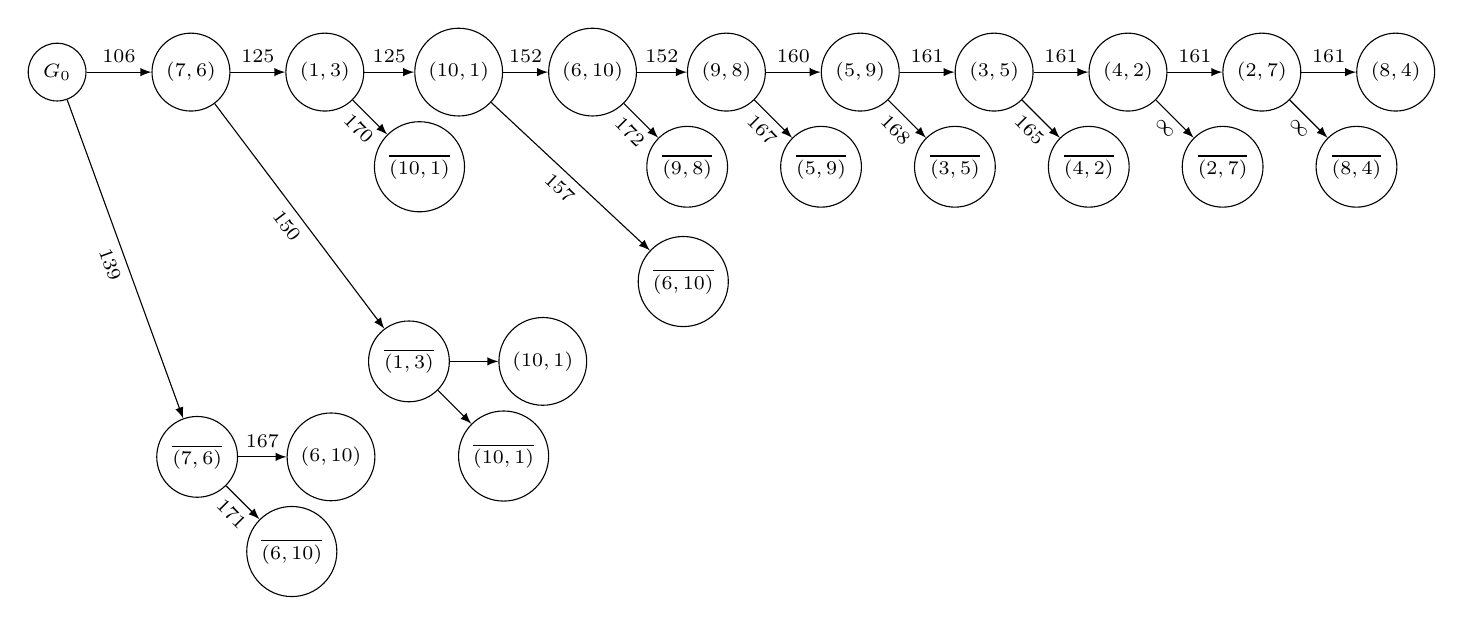
\begin{tikzpicture}[
        grow=east, % Дерево растет слева направо
        level 1/.style = {level distance=1.70cm}, % Расстояние между уровнями
        edge from parent/.style = {draw, -latex},
        kant/.style={text width=2cm, text centered, sloped, font=\scriptsize},
        cell/.style={circle, draw, align=center, font=\scriptsize}, % Стиль узлов
    ]

    \node[cell] {$G_0$}
    child[grow=east] {node[cell] {$(7, 6)$}
            child[grow=east] {node[cell] {$(1, 3)$}
                    child[grow=east] {node[cell] {$(10, 1)$}
                            child[grow=east] {node[cell] {$(6, 10)$}
                                    child[grow=east] {node[cell] {$(9, 8)$}
                                            child[grow=east] {node[cell] {$(5, 9)$}
                                                    child[grow=east] {node[cell] {$(3, 5)$}
                                                            child[grow=east] {node[cell] {$(4, 2)$}
                                                                    child[grow=east] {node[cell] {$(2, 7)$}
                                                                            child[grow=east] {node[cell] {$(8, 4)$} edge from parent node[kant, above] {161}}
                                                                            child[grow=south east] {node[cell] {$\overline{(8, 4)}$} edge from parent node[kant, below] {$\infty$}}
                                                                            edge from parent node[kant, above] {161}}
                                                                    child[grow=south east] {node[cell] {$\overline{(2, 7)}$} edge from parent node[kant, below] {$\infty$}}
                                                                    edge from parent node[kant, above] {161}}
                                                            child[grow=south east] {node[cell] {$\overline{(4, 2)}$} edge from parent node[kant, below] {165}}
                                                            edge from parent node[kant, above] {161}}
                                                    child[grow=south east] {node[cell] {$\overline{(3, 5)}$} edge from parent node[kant, below] {168}}
                                                    edge from parent node[kant, above] {160}}
                                            child[grow=south east] {node[cell] {$\overline{(5, 9)}$} edge from parent node[kant, below] {167}}
                                            edge from parent node[kant, above] {152}}
                                    child[grow=south east] {node[cell] {$\overline{(9, 8)}$} edge from parent node[kant, below] {172}}
                                    edge from parent node[kant, above] {152}}
                            child[grow=317, level distance=3.9cm] {node[cell] {$\overline{(6, 10)}$} edge from parent node[kant, below] {157}}
                            edge from parent node[kant, above] {125}}
                    child[grow=south east] {node[cell] {$\overline{(10, 1)}$} edge from parent node[kant, below] {170}}
                    edge from parent node[kant, above] {125}}
            child[grow=307, level distance=4.6cm] {node[cell] {$\overline{(1, 3)}$}
                    child[grow=east, level distance=1.7cm]{node[cell] {$(10, 1)$}}
                    child[grow=south east, level distance=1.7cm]{node[cell] {$\overline{(10, 1)}$}}
                    edge from parent node[kant, below] {150}}
            edge from parent node[kant, above] {106}}
    child[grow=290, level distance=5.2cm] {node[cell] {$\overline{(7, 6)}$}
            child[grow=east, level distance=1.7cm] {node[cell] {$(6, 10)$} edge from parent node[kant, above] {167}}
            child[grow=south east, level distance=1.7cm] {node[cell] {$\overline{(6, 10)}$} edge from parent node[kant, below] {171}}
            edge from parent node[kant, below] {139}};
\end{tikzpicture}

Найдём оценку множества $\overline{(10, 1)}$: $w(\overline{(10, 1)}) = w(\overline{(1, 3)}) + Q_{10, 1} = 150 + 41 = 191$.

Находим оценку множества $(10, 1)$. Для этого нужно вычеркнуть из таблицы строку 10 и столбец 1. А также исключить циклы: поставить $\infty$ в ячейку $(1, 10)$, чтобы не возникло цикла $10 \to 1 \to 10$. И редуцировать эту таблицу.

\[
    \begin{array}{|>{\columncolor{lightgray}}c|c|c|c|c|c|c|c|c|>{\columncolor{LightBlue}}c|}
        \hline \rowcolor{lightgray}
        \text{Город} & 2      & 3      & 4      & 5      & 7      & 8      & 9      & 10     & \text{min}              \\
        \hline
        1            & 20     & \infty & 15     & 0      & 16     & 30     & 4      & \infty & 0                       \\
        \hline
        2            & \infty & 20     & 1      & 16     & 0      & 86     & 14     & 36     & 0                       \\
        \hline
        3            & 27     & \infty & 0      & 8      & 37     & 1      & 54     & 28     & 19                      \\
        \hline
        4            & 28     & 25     & \infty & 41     & 0      & 47     & 33     & 32     & 0                       \\
        \hline
        5            & 28     & 46     & 57     & \infty & 44     & 0      & 0      & 66     & 0                       \\
        \hline
        6            & 0      & 0      & 87     & 54     & \infty & 88     & 37     & 0      & 0                       \\
        \hline
        8            & 32     & 0      & 0      & 0      & 2      & \infty & 77     & 61     & 0                       \\
        \hline
        9            & 60     & 28     & 20     & 56     & 86     & 0      & \infty & 34     & 0                       \\
        \hline \rowcolor{LightBlue}
        \text{min}   & 0      & 0      & 0      & 0      & 0      & 0      & 0      & 0      & \cellcolor{Chocolate}19 \\
        \hline
    \end{array}
\]

$h = 19$. Это значит, что $w((10, 1)) = w(\overline{(1, 3)}) + h = 150 + 19 = 169$.

$w(\overline{(10, 1)}) = 191$, $w((10, 1)) = 169$. Заметим, что все они больше полученной нами ранее оценки $w((8, 4)) = 161$. Это значит, что мы можем остановить процесс ветвления для тупиковой ветви $\overline{(1, 3)}$.

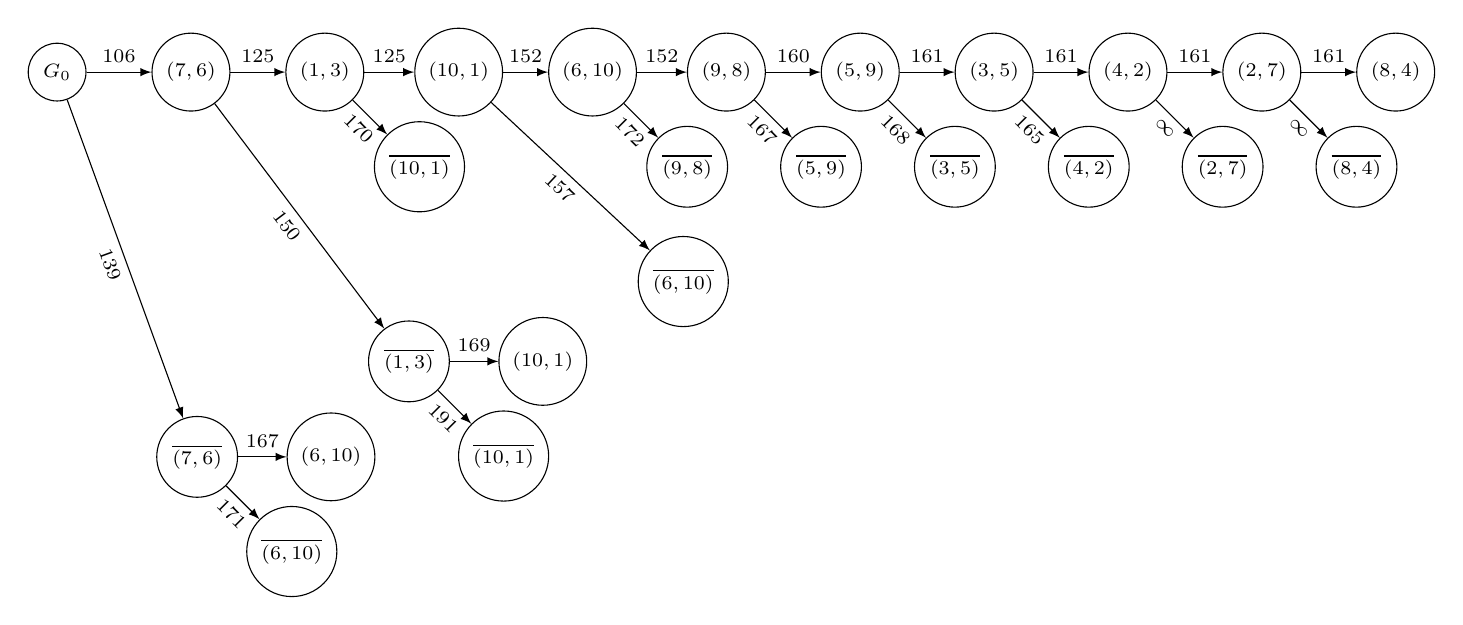
\begin{tikzpicture}[
        grow=east, % Дерево растет слева направо
        level 1/.style = {level distance=1.70cm}, % Расстояние между уровнями
        edge from parent/.style = {draw, -latex},
        kant/.style={text width=2cm, text centered, sloped, font=\scriptsize},
        cell/.style={circle, draw, align=center, font=\scriptsize}, % Стиль узлов
    ]

    \node[cell] {$G_0$}
    child[grow=east] {node[cell] {$(7, 6)$}
            child[grow=east] {node[cell] {$(1, 3)$}
                    child[grow=east] {node[cell] {$(10, 1)$}
                            child[grow=east] {node[cell] {$(6, 10)$}
                                    child[grow=east] {node[cell] {$(9, 8)$}
                                            child[grow=east] {node[cell] {$(5, 9)$}
                                                    child[grow=east] {node[cell] {$(3, 5)$}
                                                            child[grow=east] {node[cell] {$(4, 2)$}
                                                                    child[grow=east] {node[cell] {$(2, 7)$}
                                                                            child[grow=east] {node[cell] {$(8, 4)$} edge from parent node[kant, above] {161}}
                                                                            child[grow=south east] {node[cell] {$\overline{(8, 4)}$} edge from parent node[kant, below] {$\infty$}}
                                                                            edge from parent node[kant, above] {161}}
                                                                    child[grow=south east] {node[cell] {$\overline{(2, 7)}$} edge from parent node[kant, below] {$\infty$}}
                                                                    edge from parent node[kant, above] {161}}
                                                            child[grow=south east] {node[cell] {$\overline{(4, 2)}$} edge from parent node[kant, below] {165}}
                                                            edge from parent node[kant, above] {161}}
                                                    child[grow=south east] {node[cell] {$\overline{(3, 5)}$} edge from parent node[kant, below] {168}}
                                                    edge from parent node[kant, above] {160}}
                                            child[grow=south east] {node[cell] {$\overline{(5, 9)}$} edge from parent node[kant, below] {167}}
                                            edge from parent node[kant, above] {152}}
                                    child[grow=south east] {node[cell] {$\overline{(9, 8)}$} edge from parent node[kant, below] {172}}
                                    edge from parent node[kant, above] {152}}
                            child[grow=317, level distance=3.9cm] {node[cell] {$\overline{(6, 10)}$} edge from parent node[kant, below] {157}}
                            edge from parent node[kant, above] {125}}
                    child[grow=south east] {node[cell] {$\overline{(10, 1)}$} edge from parent node[kant, below] {170}}
                    edge from parent node[kant, above] {125}}
            child[grow=307, level distance=4.6cm] {node[cell] {$\overline{(1, 3)}$}
                    child[grow=east, level distance=1.7cm]{node[cell] {$(10, 1)$} edge from parent node[kant, above] {169}}
                    child[grow=south east, level distance=1.7cm]{node[cell] {$\overline{(10, 1)}$} edge from parent node[kant, below] {191}}
                    edge from parent node[kant, below] {150}}
            edge from parent node[kant, above] {106}}
    child[grow=290, level distance=5.2cm] {node[cell] {$\overline{(7, 6)}$}
            child[grow=east, level distance=1.7cm] {node[cell] {$(6, 10)$} edge from parent node[kant, above] {167}}
            child[grow=south east, level distance=1.7cm] {node[cell] {$\overline{(6, 10)}$} edge from parent node[kant, below] {171}}
            edge from parent node[kant, below] {139}};
\end{tikzpicture}

Далее ветвим $\overline{(6, 10)}$. Для этого в таблицу для $(10, 1)$ поставим $\infty$ в ячейку $(6, 10)$:

\[
    \begin{array}{|>{\columncolor{lightgray}}c|c|c|c|c|c|c|c|>{\columncolor{LightBlue}}c|}
        \hline \rowcolor{lightgray}
        \text{Город} & 2      & 4      & 5      & 7      & 8      & 9      & 10     & \text{min}              \\
        \hline
        2            & \infty & 1      & 16     & 0      & 86     & 14     & 36     & 0                       \\
        \hline
        3            & 27     & 0      & 8      & 37     & 1      & 54     & \infty & 0                       \\
        \hline
        4            & 28     & \infty & 41     & 0      & 47     & 33     & 32     & 0                       \\
        \hline
        5            & 28     & 57     & \infty & 44     & 0      & 0      & 66     & 0                       \\
        \hline
        6            & 0      & 87     & 54     & \infty & 88     & 37     & \infty & 0                       \\
        \hline
        8            & 32     & 0      & 0      & 2      & \infty & 77     & 61     & 0                       \\
        \hline
        9            & 60     & 20     & 56     & 86     & 0      & \infty & 34     & 0                       \\
        \hline \rowcolor{LightBlue}
        \text{min}   & 0      & 0      & 0      & 0      & 0      & 0      & 32     & \cellcolor{Chocolate}32 \\
        \hline
    \end{array}
\]

И потом проведём процесс редуцирования:

\[
    \begin{array}{|>{\columncolor{lightgray}}c|c|c|c|c|c|c|c|>{\columncolor{LightBlue}}c|}
        \hline \rowcolor{lightgray}
        \text{Город} & 2      & 4      & 5      & 7      & 8      & 9      & 10     & \text{min}              \\
        \hline
        2            & \infty & 1      & 16     & 0      & 86     & 14     & 4      & 0                       \\
        \hline
        3            & 27     & 0      & 8      & 37     & 1      & 54     & \infty & 0                       \\
        \hline
        4            & 28     & \infty & 41     & 0      & 47     & 33     & 0      & 0                       \\
        \hline
        5            & 28     & 57     & \infty & 44     & 0      & 0      & 34     & 0                       \\
        \hline
        6            & 0      & 87     & 54     & \infty & 88     & 37     & \infty & 0                       \\
        \hline
        8            & 32     & 0      & 0      & 2      & \infty & 77     & 29     & 0                       \\
        \hline
        9            & 60     & 20     & 56     & 86     & 0      & \infty & 2      & 0                       \\
        \hline \rowcolor{LightBlue}
        \text{min}   & 0      & 0      & 0      & 0      & 0      & 0      & 32     & \cellcolor{Chocolate}32 \\
        \hline
    \end{array}
\]

Претенденты на ветвление:

\[
    \begin{array}{|>{\columncolor{lightgray}}c|c|c|c|c|c|c|c|c|c|c|c|c|c|}
        \hline
        S      & (2, 7) & (3, 4) & (4, 7) & (4, 10) & (5, 8) & (5, 9) & (6, 2) & (8, 4) & (8, 5) & (9, 8) \\
        \hline
        d_i    & 1      & 1      & 0      & 0       & 0      & 0      & 37     & 0      & 0      & 2      \\
        \hline
        d_j    & 0      & 0      & 0      & 2       & 0      & 14     & 27     & 0      & 8      & 0      \\
        \hline
        Q_{ij} & 1      & 1      & 0      & 2       & 0      & 14     & 64     & 0      & 8      & 2      \\
        \hline
    \end{array}
\]

$\max Q_{ij} = Q_{6, 2} = 64$. Ветвление производим по элементу $(6, 2)$.

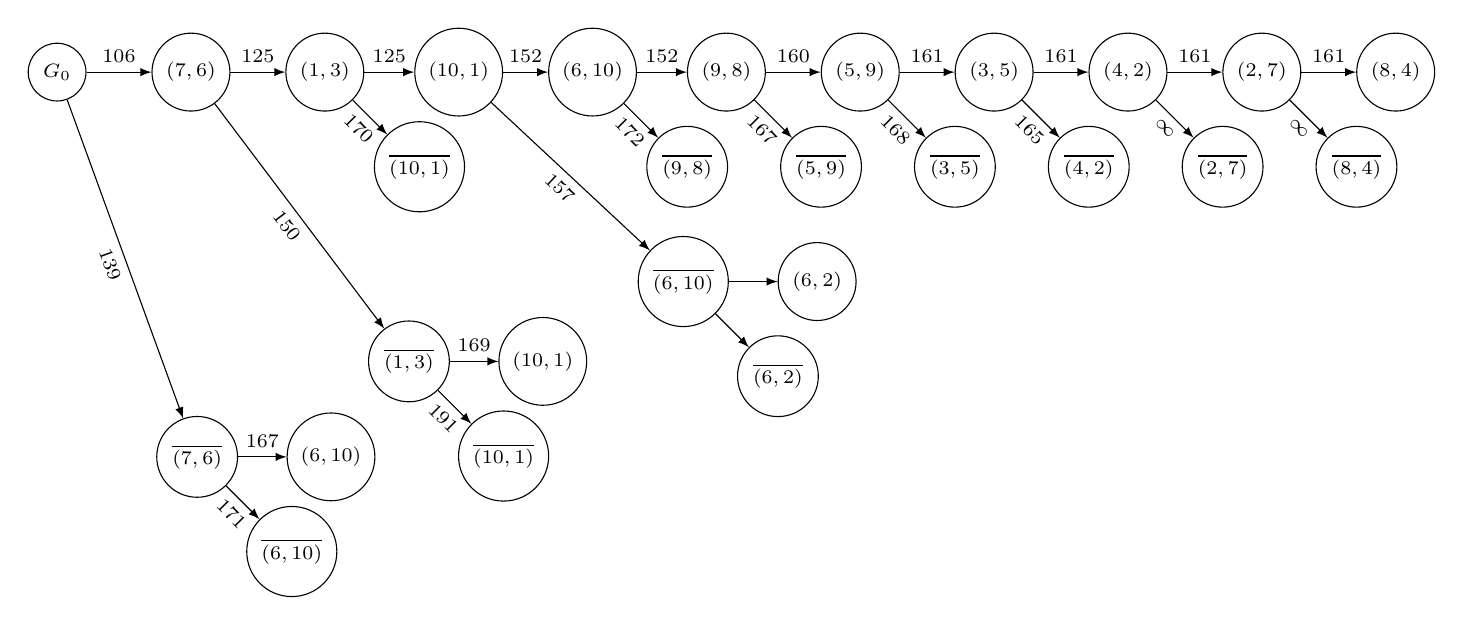
\begin{tikzpicture}[
        grow=east, % Дерево растет слева направо
        level 1/.style = {level distance=1.70cm}, % Расстояние между уровнями
        edge from parent/.style = {draw, -latex},
        kant/.style={text width=2cm, text centered, sloped, font=\scriptsize},
        cell/.style={circle, draw, align=center, font=\scriptsize}, % Стиль узлов
    ]

    \node[cell] {$G_0$}
    child[grow=east] {node[cell] {$(7, 6)$}
            child[grow=east] {node[cell] {$(1, 3)$}
                    child[grow=east] {node[cell] {$(10, 1)$}
                            child[grow=east] {node[cell] {$(6, 10)$}
                                    child[grow=east] {node[cell] {$(9, 8)$}
                                            child[grow=east] {node[cell] {$(5, 9)$}
                                                    child[grow=east] {node[cell] {$(3, 5)$}
                                                            child[grow=east] {node[cell] {$(4, 2)$}
                                                                    child[grow=east] {node[cell] {$(2, 7)$}
                                                                            child[grow=east] {node[cell] {$(8, 4)$} edge from parent node[kant, above] {161}}
                                                                            child[grow=south east] {node[cell] {$\overline{(8, 4)}$} edge from parent node[kant, below] {$\infty$}}
                                                                            edge from parent node[kant, above] {161}}
                                                                    child[grow=south east] {node[cell] {$\overline{(2, 7)}$} edge from parent node[kant, below] {$\infty$}}
                                                                    edge from parent node[kant, above] {161}}
                                                            child[grow=south east] {node[cell] {$\overline{(4, 2)}$} edge from parent node[kant, below] {165}}
                                                            edge from parent node[kant, above] {161}}
                                                    child[grow=south east] {node[cell] {$\overline{(3, 5)}$} edge from parent node[kant, below] {168}}
                                                    edge from parent node[kant, above] {160}}
                                            child[grow=south east] {node[cell] {$\overline{(5, 9)}$} edge from parent node[kant, below] {167}}
                                            edge from parent node[kant, above] {152}}
                                    child[grow=south east] {node[cell] {$\overline{(9, 8)}$} edge from parent node[kant, below] {172}}
                                    edge from parent node[kant, above] {152}}
                            child[grow=317, level distance=3.9cm] {node[cell] {$\overline{(6, 10)}$}
                                    child[grow=east, level distance=1.70cm] {node[cell] {$(6, 2)$}}
                                    child[grow=south east, level distance=1.70cm] {node[cell] {$\overline{(6, 2)}$}}
                                    edge from parent node[kant, below] {157}}
                            edge from parent node[kant, above] {125}}
                    child[grow=south east] {node[cell] {$\overline{(10, 1)}$} edge from parent node[kant, below] {170}}
                    edge from parent node[kant, above] {125}}
            child[grow=307, level distance=4.6cm] {node[cell] {$\overline{(1, 3)}$}
                    child[grow=east, level distance=1.7cm]{node[cell] {$(10, 1)$} edge from parent node[kant, above] {169}}
                    child[grow=south east, level distance=1.7cm]{node[cell] {$\overline{(10, 1)}$} edge from parent node[kant, below] {191}}
                    edge from parent node[kant, below] {150}}
            edge from parent node[kant, above] {106}}
    child[grow=290, level distance=5.2cm] {node[cell] {$\overline{(7, 6)}$}
            child[grow=east, level distance=1.7cm] {node[cell] {$(6, 10)$} edge from parent node[kant, above] {167}}
            child[grow=south east, level distance=1.7cm] {node[cell] {$\overline{(6, 10)}$} edge from parent node[kant, below] {171}}
            edge from parent node[kant, below] {139}};
\end{tikzpicture}

Найдём оценку множества $\overline{(6, 2)}$: $w(\overline{(6, 2)}) = w(\overline{(6, 10)}) + Q_{6, 2} = 157 + 64 = 221$.

Находим оценку множества $(6, 2)$. Для этого нужно вычеркнуть из таблицы строку 6 и столбец 2, а также исключить циклы: поставить $\infty$ в ячейку $(2, 7)$, чтобы не возникло цикла $7 \to 6 \to 2 \to 7$.

\[
    \begin{array}{|>{\columncolor{lightgray}}c|c|c|c|c|c|c|>{\columncolor{LightBlue}}c|}
        \hline \rowcolor{lightgray}
        \text{Город} & 4      & 5      & 7  & 8      & 9      & 10     & \text{min}             \\
        \hline
        2            & 1      & 16     & 0  & 86     & 14     & 4      & 0                      \\
        \hline
        3            & 0      & 8      & 37 & 1      & 54     & \infty & 0                      \\
        \hline
        4            & \infty & 41     & 0  & 47     & 33     & 0      & 0                      \\
        \hline
        5            & 57     & \infty & 44 & 0      & 0      & 34     & 0                      \\
        \hline
        8            & 0      & 0      & 2  & \infty & 77     & 29     & 0                      \\
        \hline
        9            & 20     & 56     & 86 & 0      & \infty & 2      & 0                      \\
        \hline \rowcolor{LightBlue}
        \text{min}   & 0      & 0      & 0  & 0      & 0      & 0      & \cellcolor{Chocolate}0 \\
        \hline
    \end{array}
\]

$h = 0$. Это значит, что $w((6, 2)) = w(\overline{(6, 10)}) + h = 157 + 0 = 157$.

$w(\overline{(6, 2)}) = 221$, $w((6, 2)) = 157$. Выбираем ветвь с меньшей оценкой, то есть $(6, 2)$.

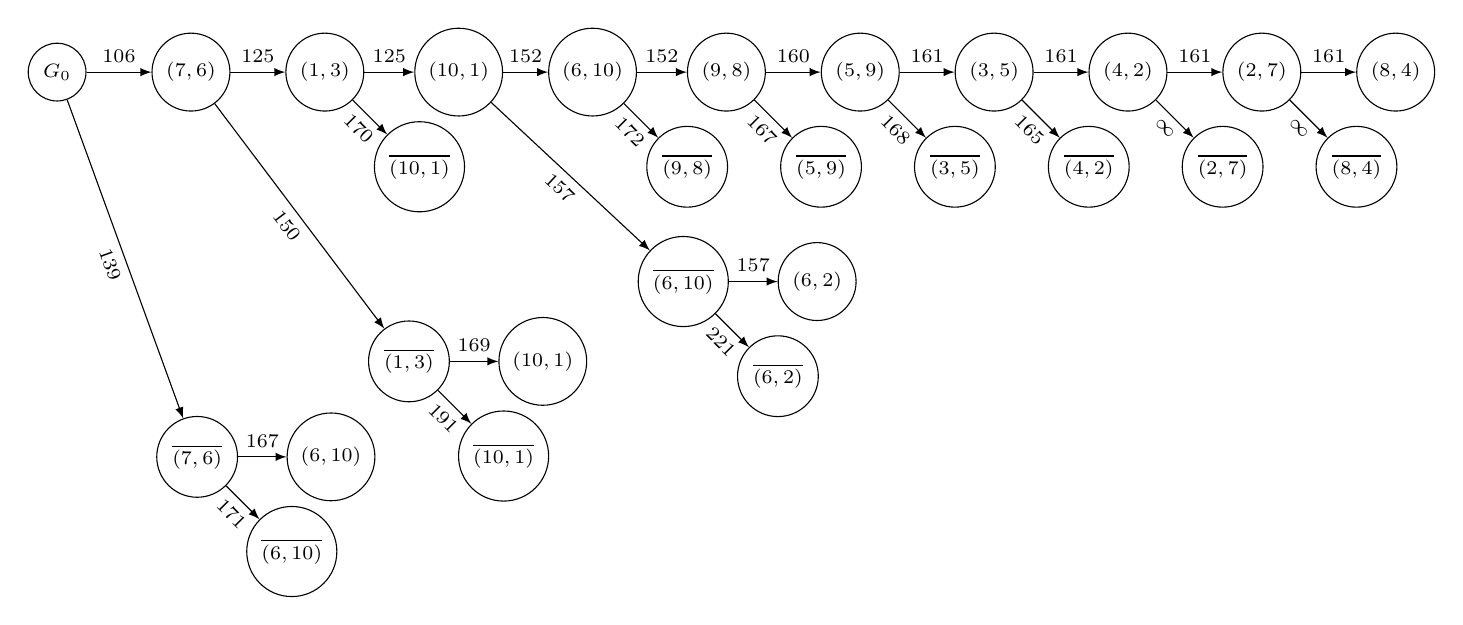
\begin{tikzpicture}[
        grow=east, % Дерево растет слева направо
        level 1/.style = {level distance=1.70cm}, % Расстояние между уровнями
        edge from parent/.style = {draw, -latex},
        kant/.style={text width=2cm, text centered, sloped, font=\scriptsize},
        cell/.style={circle, draw, align=center, font=\scriptsize}, % Стиль узлов
    ]

    \node[cell] {$G_0$}
    child[grow=east] {node[cell] {$(7, 6)$}
            child[grow=east] {node[cell] {$(1, 3)$}
                    child[grow=east] {node[cell] {$(10, 1)$}
                            child[grow=east] {node[cell] {$(6, 10)$}
                                    child[grow=east] {node[cell] {$(9, 8)$}
                                            child[grow=east] {node[cell] {$(5, 9)$}
                                                    child[grow=east] {node[cell] {$(3, 5)$}
                                                            child[grow=east] {node[cell] {$(4, 2)$}
                                                                    child[grow=east] {node[cell] {$(2, 7)$}
                                                                            child[grow=east] {node[cell] {$(8, 4)$} edge from parent node[kant, above] {161}}
                                                                            child[grow=south east] {node[cell] {$\overline{(8, 4)}$} edge from parent node[kant, below] {$\infty$}}
                                                                            edge from parent node[kant, above] {161}}
                                                                    child[grow=south east] {node[cell] {$\overline{(2, 7)}$} edge from parent node[kant, below] {$\infty$}}
                                                                    edge from parent node[kant, above] {161}}
                                                            child[grow=south east] {node[cell] {$\overline{(4, 2)}$} edge from parent node[kant, below] {165}}
                                                            edge from parent node[kant, above] {161}}
                                                    child[grow=south east] {node[cell] {$\overline{(3, 5)}$} edge from parent node[kant, below] {168}}
                                                    edge from parent node[kant, above] {160}}
                                            child[grow=south east] {node[cell] {$\overline{(5, 9)}$} edge from parent node[kant, below] {167}}
                                            edge from parent node[kant, above] {152}}
                                    child[grow=south east] {node[cell] {$\overline{(9, 8)}$} edge from parent node[kant, below] {172}}
                                    edge from parent node[kant, above] {152}}
                            child[grow=317, level distance=3.9cm] {node[cell] {$\overline{(6, 10)}$}
                                    child[grow=east, level distance=1.70cm] {node[cell] {$(6, 2)$} edge from parent node[kant, above] {157}}
                                    child[grow=south east, level distance=1.70cm] {node[cell] {$\overline{(6, 2)}$} edge from parent node[kant, below] {221}}
                                    edge from parent node[kant, below] {157}}
                            edge from parent node[kant, above] {125}}
                    child[grow=south east] {node[cell] {$\overline{(10, 1)}$} edge from parent node[kant, below] {170}}
                    edge from parent node[kant, above] {125}}
            child[grow=307, level distance=4.6cm] {node[cell] {$\overline{(1, 3)}$}
                    child[grow=east, level distance=1.7cm]{node[cell] {$(10, 1)$} edge from parent node[kant, above] {169}}
                    child[grow=south east, level distance=1.7cm]{node[cell] {$\overline{(10, 1)}$} edge from parent node[kant, below] {191}}
                    edge from parent node[kant, below] {150}}
            edge from parent node[kant, above] {106}}
    child[grow=290, level distance=5.2cm] {node[cell] {$\overline{(7, 6)}$}
            child[grow=east, level distance=1.7cm] {node[cell] {$(6, 10)$} edge from parent node[kant, above] {167}}
            child[grow=south east, level distance=1.7cm] {node[cell] {$\overline{(6, 10)}$} edge from parent node[kant, below] {171}}
            edge from parent node[kant, below] {139}};
\end{tikzpicture}

Найдём претендентов на ветвление:

\[
    \begin{array}{|>{\columncolor{lightgray}}c|c|c|c|c|c|c|c|c|c|c|c|c|c|}
        \hline
        S      & (2, 7) & (3, 4) & (4, 7) & (4, 10) & (5, 8) & (5, 9) & (8, 4) & (8, 5) & (9, 8) \\
        \hline
        d_i    & 1      & 1      & 0      & 0       & 0      & 0      & 0      & 0      & 2      \\
        \hline
        d_j    & 0      & 0      & 0      & 2       & 0      & 14     & 0      & 8      & 0      \\
        \hline
        Q_{ij} & 1      & 1      & 0      & 2       & 0      & 14     & 0      & 8      & 2      \\
        \hline
    \end{array}
\]

$\max Q_{ij} = Q_{5, 9} = 14$. Ветвление производим по элементу $(5, 9)$.

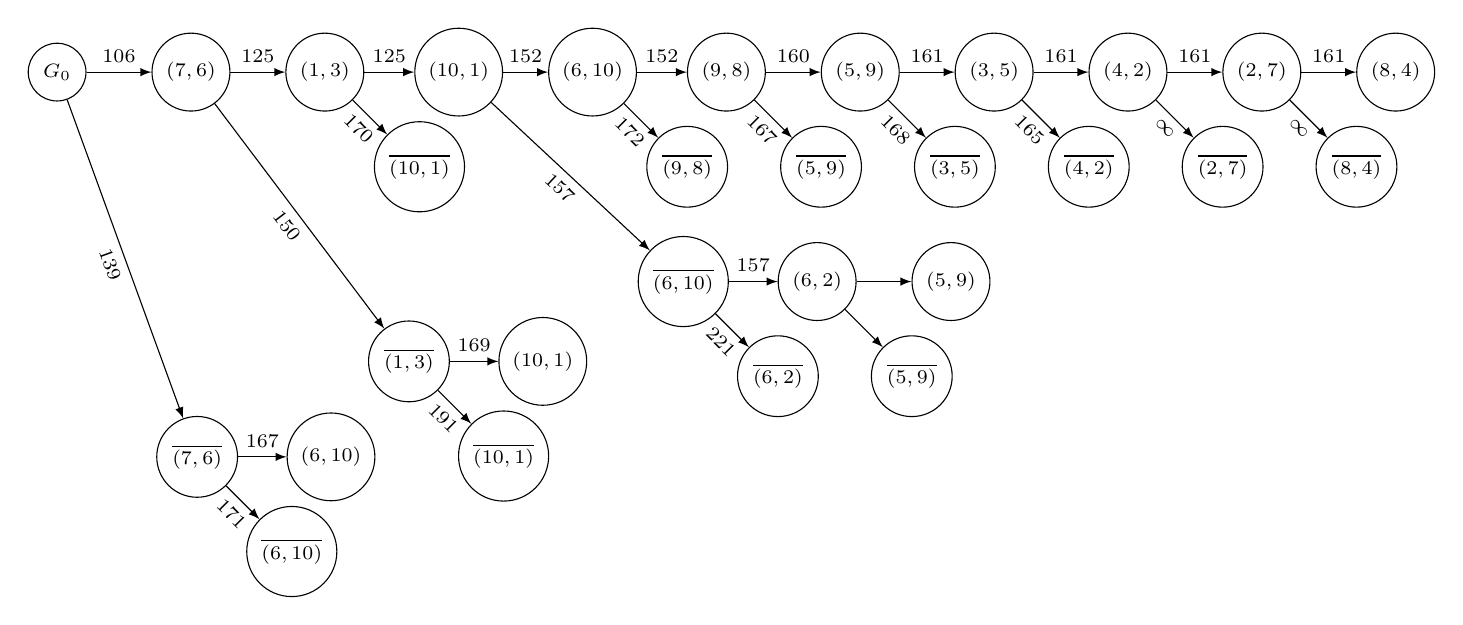
\begin{tikzpicture}[
        grow=east, % Дерево растет слева направо
        level 1/.style = {level distance=1.70cm}, % Расстояние между уровнями
        edge from parent/.style = {draw, -latex},
        kant/.style={text width=2cm, text centered, sloped, font=\scriptsize},
        cell/.style={circle, draw, align=center, font=\scriptsize}, % Стиль узлов
    ]

    \node[cell] {$G_0$}
    child[grow=east] {node[cell] {$(7, 6)$}
            child[grow=east] {node[cell] {$(1, 3)$}
                    child[grow=east] {node[cell] {$(10, 1)$}
                            child[grow=east] {node[cell] {$(6, 10)$}
                                    child[grow=east] {node[cell] {$(9, 8)$}
                                            child[grow=east] {node[cell] {$(5, 9)$}
                                                    child[grow=east] {node[cell] {$(3, 5)$}
                                                            child[grow=east] {node[cell] {$(4, 2)$}
                                                                    child[grow=east] {node[cell] {$(2, 7)$}
                                                                            child[grow=east] {node[cell] {$(8, 4)$} edge from parent node[kant, above] {161}}
                                                                            child[grow=south east] {node[cell] {$\overline{(8, 4)}$} edge from parent node[kant, below] {$\infty$}}
                                                                            edge from parent node[kant, above] {161}}
                                                                    child[grow=south east] {node[cell] {$\overline{(2, 7)}$} edge from parent node[kant, below] {$\infty$}}
                                                                    edge from parent node[kant, above] {161}}
                                                            child[grow=south east] {node[cell] {$\overline{(4, 2)}$} edge from parent node[kant, below] {165}}
                                                            edge from parent node[kant, above] {161}}
                                                    child[grow=south east] {node[cell] {$\overline{(3, 5)}$} edge from parent node[kant, below] {168}}
                                                    edge from parent node[kant, above] {160}}
                                            child[grow=south east] {node[cell] {$\overline{(5, 9)}$} edge from parent node[kant, below] {167}}
                                            edge from parent node[kant, above] {152}}
                                    child[grow=south east] {node[cell] {$\overline{(9, 8)}$} edge from parent node[kant, below] {172}}
                                    edge from parent node[kant, above] {152}}
                            child[grow=317, level distance=3.9cm] {node[cell] {$\overline{(6, 10)}$}
                                    child[grow=east, level distance=1.70cm] {node[cell] {$(6, 2)$}
                                            child[grow=east] {node[cell] {$(5, 9)$}}
                                            child[grow=south east] {node[cell] {$\overline{(5, 9)}$}}
                                            edge from parent node[kant, above] {157}}
                                    child[grow=south east, level distance=1.70cm] {node[cell] {$\overline{(6, 2)}$} edge from parent node[kant, below] {221}}
                                    edge from parent node[kant, below] {157}}
                            edge from parent node[kant, above] {125}}
                    child[grow=south east] {node[cell] {$\overline{(10, 1)}$} edge from parent node[kant, below] {170}}
                    edge from parent node[kant, above] {125}}
            child[grow=307, level distance=4.6cm] {node[cell] {$\overline{(1, 3)}$}
                    child[grow=east, level distance=1.7cm]{node[cell] {$(10, 1)$} edge from parent node[kant, above] {169}}
                    child[grow=south east, level distance=1.7cm]{node[cell] {$\overline{(10, 1)}$} edge from parent node[kant, below] {191}}
                    edge from parent node[kant, below] {150}}
            edge from parent node[kant, above] {106}}
    child[grow=290, level distance=5.2cm] {node[cell] {$\overline{(7, 6)}$}
            child[grow=east, level distance=1.7cm] {node[cell] {$(6, 10)$} edge from parent node[kant, above] {167}}
            child[grow=south east, level distance=1.7cm] {node[cell] {$\overline{(6, 10)}$} edge from parent node[kant, below] {171}}
            edge from parent node[kant, below] {139}};
\end{tikzpicture}

Найдём оценку множества $\overline{(5, 9)}$: $w(\overline{(5, 9)}) = w(\overline{(6, 10)}) + Q_{5, 9} = 157 + 14 = 171$.

Находим оценку множества $(5, 9)$. Для этого нужно вычеркнуть из таблицы строку 5 и столбец 9, а также исключить циклы: поставить $\infty$ в ячейку $(9, 5)$, чтобы не возникло цикла $5 \to 9 \to 5$.

\[
    \begin{array}{|>{\columncolor{lightgray}}c|c|c|c|c|c|>{\columncolor{LightBlue}}c|}
        \hline \rowcolor{lightgray}
        \text{Город} & 4      & 5      & 7  & 8      & 10     & \text{min}             \\
        \hline
        2            & 1      & 16     & 0  & 86     & 4      & 0                      \\
        \hline
        3            & 0      & 8      & 37 & 1      & \infty & 0                      \\
        \hline
        4            & \infty & 41     & 0  & 47     & 0      & 0                      \\
        \hline
        8            & 0      & 0      & 2  & \infty & 29     & 0                      \\
        \hline
        9            & 20     & \infty & 86 & 0      & 2      & 0                      \\
        \hline \rowcolor{LightBlue}
        \text{min}   & 0      & 0      & 0  & 0      & 0      & \cellcolor{Chocolate}0 \\
        \hline
    \end{array}
\]

$h = 0$. Это значит, что $w((5, 9)) = w(\overline{(6, 10)}) + h = 157 + 0 = 157$.

$w(\overline{(5, 9)}) = 171$, $w((5, 9)) = 157$. Выбираем ветвь с меньшей оценкой, то есть $(5, 9)$.

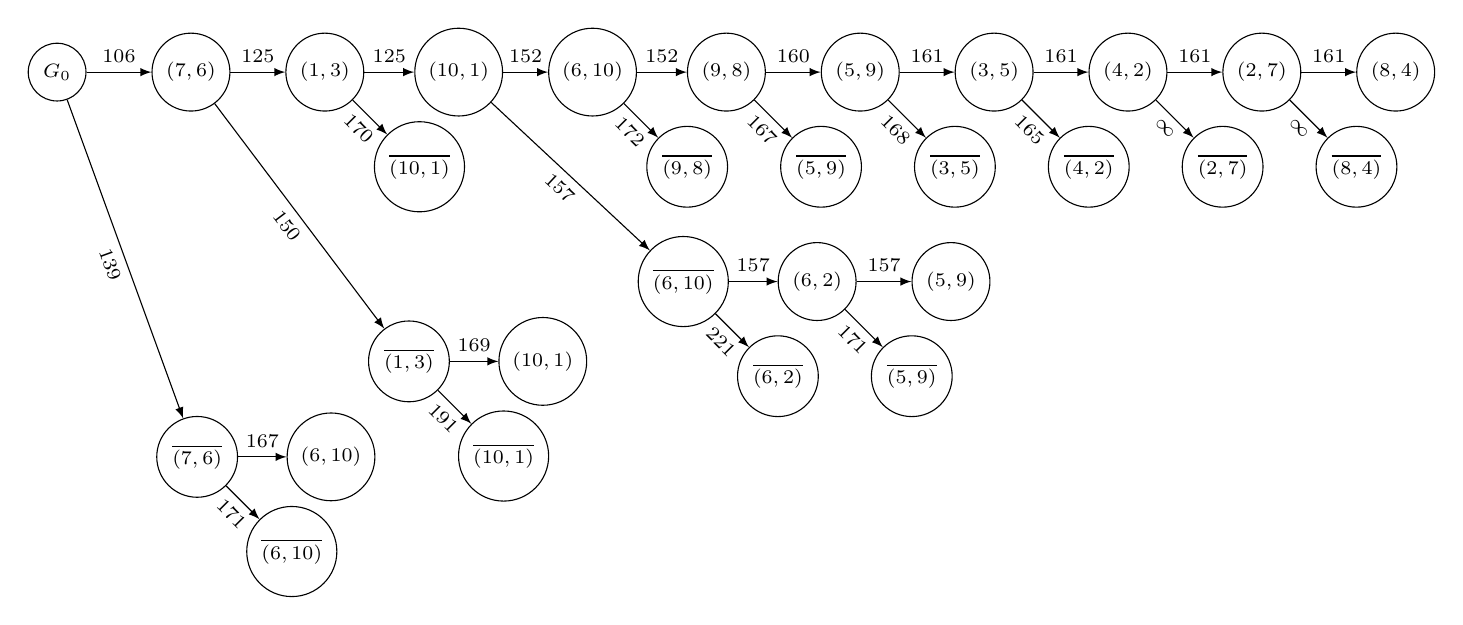
\begin{tikzpicture}[
        grow=east, % Дерево растет слева направо
        level 1/.style = {level distance=1.70cm}, % Расстояние между уровнями
        edge from parent/.style = {draw, -latex},
        kant/.style={text width=2cm, text centered, sloped, font=\scriptsize},
        cell/.style={circle, draw, align=center, font=\scriptsize}, % Стиль узлов
    ]

    \node[cell] {$G_0$}
    child[grow=east] {node[cell] {$(7, 6)$}
            child[grow=east] {node[cell] {$(1, 3)$}
                    child[grow=east] {node[cell] {$(10, 1)$}
                            child[grow=east] {node[cell] {$(6, 10)$}
                                    child[grow=east] {node[cell] {$(9, 8)$}
                                            child[grow=east] {node[cell] {$(5, 9)$}
                                                    child[grow=east] {node[cell] {$(3, 5)$}
                                                            child[grow=east] {node[cell] {$(4, 2)$}
                                                                    child[grow=east] {node[cell] {$(2, 7)$}
                                                                            child[grow=east] {node[cell] {$(8, 4)$} edge from parent node[kant, above] {161}}
                                                                            child[grow=south east] {node[cell] {$\overline{(8, 4)}$} edge from parent node[kant, below] {$\infty$}}
                                                                            edge from parent node[kant, above] {161}}
                                                                    child[grow=south east] {node[cell] {$\overline{(2, 7)}$} edge from parent node[kant, below] {$\infty$}}
                                                                    edge from parent node[kant, above] {161}}
                                                            child[grow=south east] {node[cell] {$\overline{(4, 2)}$} edge from parent node[kant, below] {165}}
                                                            edge from parent node[kant, above] {161}}
                                                    child[grow=south east] {node[cell] {$\overline{(3, 5)}$} edge from parent node[kant, below] {168}}
                                                    edge from parent node[kant, above] {160}}
                                            child[grow=south east] {node[cell] {$\overline{(5, 9)}$} edge from parent node[kant, below] {167}}
                                            edge from parent node[kant, above] {152}}
                                    child[grow=south east] {node[cell] {$\overline{(9, 8)}$} edge from parent node[kant, below] {172}}
                                    edge from parent node[kant, above] {152}}
                            child[grow=317, level distance=3.9cm] {node[cell] {$\overline{(6, 10)}$}
                                    child[grow=east, level distance=1.70cm] {node[cell] {$(6, 2)$}
                                            child[grow=east] {node[cell] {$(5, 9)$} edge from parent node[kant, above] {157}}
                                            child[grow=south east] {node[cell] {$\overline{(5, 9)}$} edge from parent node[kant, below] {171}}
                                            edge from parent node[kant, above] {157}}
                                    child[grow=south east, level distance=1.70cm] {node[cell] {$\overline{(6, 2)}$} edge from parent node[kant, below] {221}}
                                    edge from parent node[kant, below] {157}}
                            edge from parent node[kant, above] {125}}
                    child[grow=south east] {node[cell] {$\overline{(10, 1)}$} edge from parent node[kant, below] {170}}
                    edge from parent node[kant, above] {125}}
            child[grow=307, level distance=4.6cm] {node[cell] {$\overline{(1, 3)}$}
                    child[grow=east, level distance=1.7cm]{node[cell] {$(10, 1)$} edge from parent node[kant, above] {169}}
                    child[grow=south east, level distance=1.7cm]{node[cell] {$\overline{(10, 1)}$} edge from parent node[kant, below] {191}}
                    edge from parent node[kant, below] {150}}
            edge from parent node[kant, above] {106}}
    child[grow=290, level distance=5.2cm] {node[cell] {$\overline{(7, 6)}$}
            child[grow=east, level distance=1.7cm] {node[cell] {$(6, 10)$} edge from parent node[kant, above] {167}}
            child[grow=south east, level distance=1.7cm] {node[cell] {$\overline{(6, 10)}$} edge from parent node[kant, below] {171}}
            edge from parent node[kant, below] {139}};
\end{tikzpicture}

Найдём претендентов на ветвление:

\[
    \begin{array}{|>{\columncolor{lightgray}}c|c|c|c|c|c|c|c|c|c|c|c|c|c|}
        \hline
        S      & (2, 7) & (3, 4) & (4, 7) & (4, 10) & (8, 4) & (8, 5) & (9, 8) \\
        \hline
        d_i    & 1      & 1      & 0      & 0       & 0      & 0      & 2      \\
        \hline
        d_j    & 0      & 0      & 0      & 2       & 0      & 8      & 1      \\
        \hline
        Q_{ij} & 1      & 1      & 0      & 2       & 0      & 8      & 3      \\
        \hline
    \end{array}
\]

$\max Q_{ij} = Q_{8, 5} = 8$. Ветвление производим по элементу $(8, 5)$.

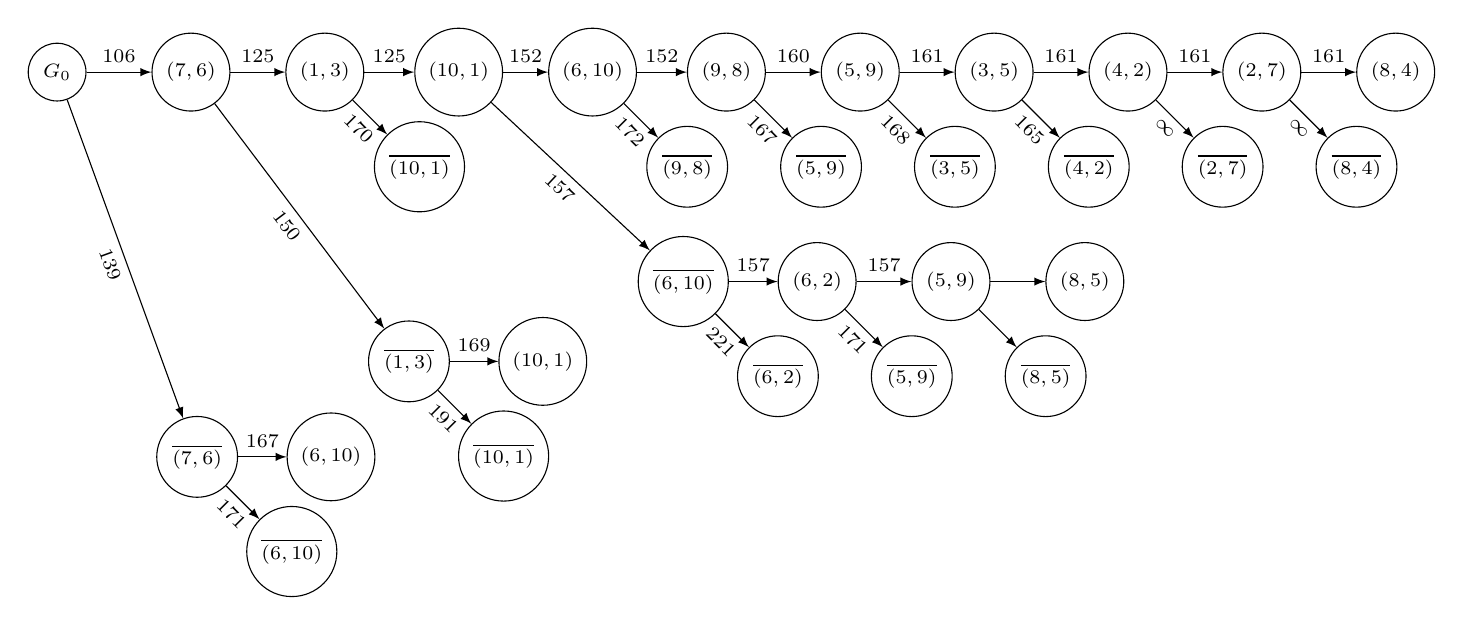
\begin{tikzpicture}[
        grow=east, % Дерево растет слева направо
        level 1/.style = {level distance=1.70cm}, % Расстояние между уровнями
        edge from parent/.style = {draw, -latex},
        kant/.style={text width=2cm, text centered, sloped, font=\scriptsize},
        cell/.style={circle, draw, align=center, font=\scriptsize}, % Стиль узлов
    ]

    \node[cell] {$G_0$}
    child[grow=east] {node[cell] {$(7, 6)$}
            child[grow=east] {node[cell] {$(1, 3)$}
                    child[grow=east] {node[cell] {$(10, 1)$}
                            child[grow=east] {node[cell] {$(6, 10)$}
                                    child[grow=east] {node[cell] {$(9, 8)$}
                                            child[grow=east] {node[cell] {$(5, 9)$}
                                                    child[grow=east] {node[cell] {$(3, 5)$}
                                                            child[grow=east] {node[cell] {$(4, 2)$}
                                                                    child[grow=east] {node[cell] {$(2, 7)$}
                                                                            child[grow=east] {node[cell] {$(8, 4)$} edge from parent node[kant, above] {161}}
                                                                            child[grow=south east] {node[cell] {$\overline{(8, 4)}$} edge from parent node[kant, below] {$\infty$}}
                                                                            edge from parent node[kant, above] {161}}
                                                                    child[grow=south east] {node[cell] {$\overline{(2, 7)}$} edge from parent node[kant, below] {$\infty$}}
                                                                    edge from parent node[kant, above] {161}}
                                                            child[grow=south east] {node[cell] {$\overline{(4, 2)}$} edge from parent node[kant, below] {165}}
                                                            edge from parent node[kant, above] {161}}
                                                    child[grow=south east] {node[cell] {$\overline{(3, 5)}$} edge from parent node[kant, below] {168}}
                                                    edge from parent node[kant, above] {160}}
                                            child[grow=south east] {node[cell] {$\overline{(5, 9)}$} edge from parent node[kant, below] {167}}
                                            edge from parent node[kant, above] {152}}
                                    child[grow=south east] {node[cell] {$\overline{(9, 8)}$} edge from parent node[kant, below] {172}}
                                    edge from parent node[kant, above] {152}}
                            child[grow=317, level distance=3.9cm] {node[cell] {$\overline{(6, 10)}$}
                                    child[grow=east, level distance=1.70cm] {node[cell] {$(6, 2)$}
                                            child[grow=east] {node[cell] {$(5, 9)$}
                                                    child[grow=east] {node[cell] {$(8, 5)$}}
                                                    child[grow=south east] {node[cell] {$\overline{(8, 5)}$}}
                                                    edge from parent node[kant, above] {157}}
                                            child[grow=south east] {node[cell] {$\overline{(5, 9)}$} edge from parent node[kant, below] {171}}
                                            edge from parent node[kant, above] {157}}
                                    child[grow=south east, level distance=1.70cm] {node[cell] {$\overline{(6, 2)}$} edge from parent node[kant, below] {221}}
                                    edge from parent node[kant, below] {157}}
                            edge from parent node[kant, above] {125}}
                    child[grow=south east] {node[cell] {$\overline{(10, 1)}$} edge from parent node[kant, below] {170}}
                    edge from parent node[kant, above] {125}}
            child[grow=307, level distance=4.6cm] {node[cell] {$\overline{(1, 3)}$}
                    child[grow=east, level distance=1.7cm]{node[cell] {$(10, 1)$} edge from parent node[kant, above] {169}}
                    child[grow=south east, level distance=1.7cm]{node[cell] {$\overline{(10, 1)}$} edge from parent node[kant, below] {191}}
                    edge from parent node[kant, below] {150}}
            edge from parent node[kant, above] {106}}
    child[grow=290, level distance=5.2cm] {node[cell] {$\overline{(7, 6)}$}
            child[grow=east, level distance=1.7cm] {node[cell] {$(6, 10)$} edge from parent node[kant, above] {167}}
            child[grow=south east, level distance=1.7cm] {node[cell] {$\overline{(6, 10)}$} edge from parent node[kant, below] {171}}
            edge from parent node[kant, below] {139}};
\end{tikzpicture}

Найдём оценку множества $\overline{(8, 5)}$: $w(\overline{(8, 5)}) = w((5, 9)) + Q_{8, 5} = 157 + 8 = 165$.

Находим оценку множества $(8, 5)$. Для этого нужно вычеркнуть из таблицы строку 8 и столбец 5, а также исключить циклы: поставить $\infty$ в ячейку $(9, 8)$, чтобы не возникло цикла $8 \to 5 \to 9 \to 8$.

\[
    \begin{array}{|>{\columncolor{lightgray}}c|c|c|c|c|>{\columncolor{LightBlue}}c|}
        \hline \rowcolor{lightgray}
        \text{Город} & 4      & 7  & 8      & 10     & \text{min}             \\
        \hline
        2            & 1      & 0  & 86     & 4      & 0                      \\
        \hline
        3            & 0      & 37 & 1      & \infty & 0                      \\
        \hline
        4            & \infty & 0  & 47     & 0      & 0                      \\
        \hline
        9            & 20     & 86 & \infty & 2      & 2                      \\
        \hline \rowcolor{LightBlue}
        \text{min}   & 0      & 0  & 1      & 0      & \cellcolor{Chocolate}3 \\
        \hline
    \end{array}
\]

Редуцируем таблицу:

\[
    \begin{array}{|>{\columncolor{lightgray}}c|c|c|c|c|>{\columncolor{LightBlue}}c|}
        \hline \rowcolor{lightgray}
        \text{Город} & 4      & 7  & 8      & 10     & \text{min}             \\
        \hline
        2            & 1      & 0  & 85     & 4      & 0                      \\
        \hline
        3            & 0      & 37 & 0      & \infty & 0                      \\
        \hline
        4            & \infty & 0  & 46     & 0      & 0                      \\
        \hline
        9            & 18     & 84 & \infty & 0      & 2                      \\
        \hline \rowcolor{LightBlue}
        \text{min}   & 0      & 0  & 1      & 0      & \cellcolor{Chocolate}3 \\
        \hline
    \end{array}
\]

$h = 3$. Это значит, что $w((8, 5)) = w((5, 9)) + h = 157 + 3 = 160$.

$w(\overline{(8, 5)}) = 165$, $w((8, 5)) = 160$. Выбираем ветвь с меньшей оценкой, то есть $(8, 5)$.

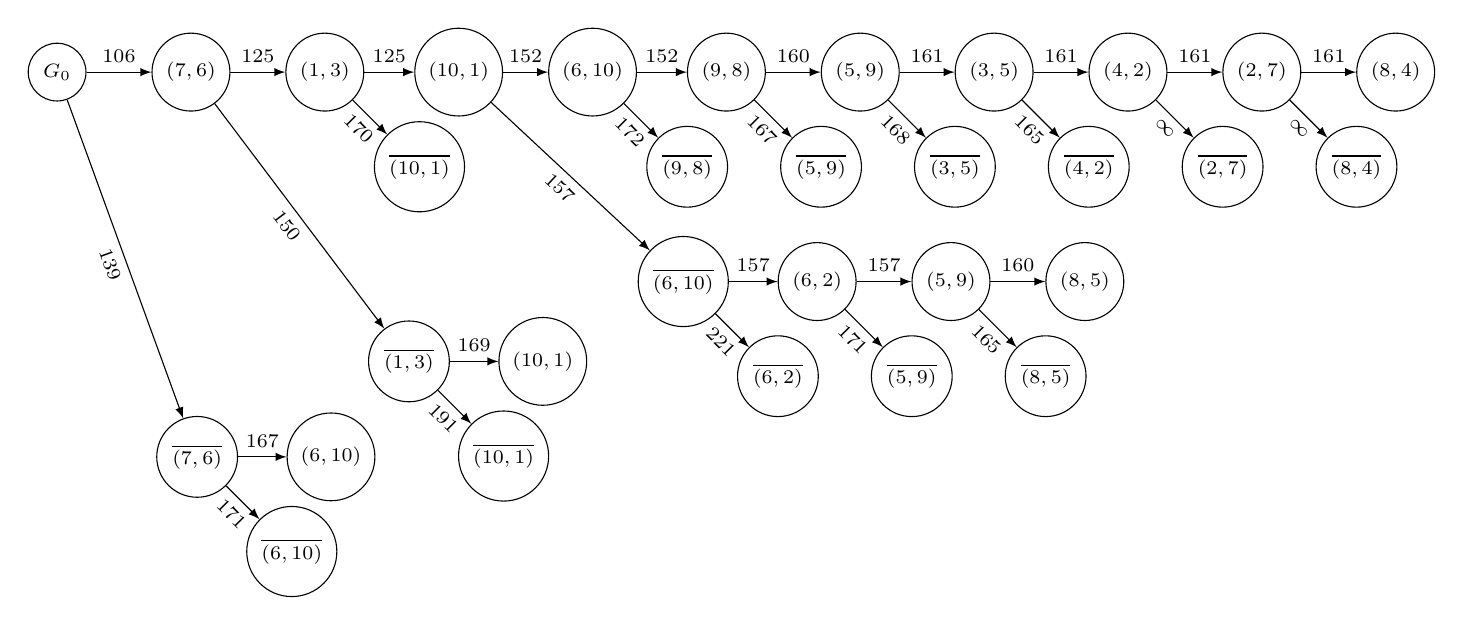
\begin{tikzpicture}[
        grow=east, % Дерево растет слева направо
        level 1/.style = {level distance=1.70cm}, % Расстояние между уровнями
        edge from parent/.style = {draw, -latex},
        kant/.style={text width=2cm, text centered, sloped, font=\scriptsize},
        cell/.style={circle, draw, align=center, font=\scriptsize}, % Стиль узлов
    ]

    \node[cell] {$G_0$}
    child[grow=east] {node[cell] {$(7, 6)$}
            child[grow=east] {node[cell] {$(1, 3)$}
                    child[grow=east] {node[cell] {$(10, 1)$}
                            child[grow=east] {node[cell] {$(6, 10)$}
                                    child[grow=east] {node[cell] {$(9, 8)$}
                                            child[grow=east] {node[cell] {$(5, 9)$}
                                                    child[grow=east] {node[cell] {$(3, 5)$}
                                                            child[grow=east] {node[cell] {$(4, 2)$}
                                                                    child[grow=east] {node[cell] {$(2, 7)$}
                                                                            child[grow=east] {node[cell] {$(8, 4)$} edge from parent node[kant, above] {161}}
                                                                            child[grow=south east] {node[cell] {$\overline{(8, 4)}$} edge from parent node[kant, below] {$\infty$}}
                                                                            edge from parent node[kant, above] {161}}
                                                                    child[grow=south east] {node[cell] {$\overline{(2, 7)}$} edge from parent node[kant, below] {$\infty$}}
                                                                    edge from parent node[kant, above] {161}}
                                                            child[grow=south east] {node[cell] {$\overline{(4, 2)}$} edge from parent node[kant, below] {165}}
                                                            edge from parent node[kant, above] {161}}
                                                    child[grow=south east] {node[cell] {$\overline{(3, 5)}$} edge from parent node[kant, below] {168}}
                                                    edge from parent node[kant, above] {160}}
                                            child[grow=south east] {node[cell] {$\overline{(5, 9)}$} edge from parent node[kant, below] {167}}
                                            edge from parent node[kant, above] {152}}
                                    child[grow=south east] {node[cell] {$\overline{(9, 8)}$} edge from parent node[kant, below] {172}}
                                    edge from parent node[kant, above] {152}}
                            child[grow=317, level distance=3.9cm] {node[cell] {$\overline{(6, 10)}$}
                                    child[grow=east, level distance=1.70cm] {node[cell] {$(6, 2)$}
                                            child[grow=east] {node[cell] {$(5, 9)$}
                                                    child[grow=east] {node[cell] {$(8, 5)$} edge from parent node[kant, above] {160}}
                                                    child[grow=south east] {node[cell] {$\overline{(8, 5)}$} edge from parent node[kant, below] {165}}
                                                    edge from parent node[kant, above] {157}}
                                            child[grow=south east] {node[cell] {$\overline{(5, 9)}$} edge from parent node[kant, below] {171}}
                                            edge from parent node[kant, above] {157}}
                                    child[grow=south east, level distance=1.70cm] {node[cell] {$\overline{(6, 2)}$} edge from parent node[kant, below] {221}}
                                    edge from parent node[kant, below] {157}}
                            edge from parent node[kant, above] {125}}
                    child[grow=south east] {node[cell] {$\overline{(10, 1)}$} edge from parent node[kant, below] {170}}
                    edge from parent node[kant, above] {125}}
            child[grow=307, level distance=4.6cm] {node[cell] {$\overline{(1, 3)}$}
                    child[grow=east, level distance=1.7cm]{node[cell] {$(10, 1)$} edge from parent node[kant, above] {169}}
                    child[grow=south east, level distance=1.7cm]{node[cell] {$\overline{(10, 1)}$} edge from parent node[kant, below] {191}}
                    edge from parent node[kant, below] {150}}
            edge from parent node[kant, above] {106}}
    child[grow=290, level distance=5.2cm] {node[cell] {$\overline{(7, 6)}$}
            child[grow=east, level distance=1.7cm] {node[cell] {$(6, 10)$} edge from parent node[kant, above] {167}}
            child[grow=south east, level distance=1.7cm] {node[cell] {$\overline{(6, 10)}$} edge from parent node[kant, below] {171}}
            edge from parent node[kant, below] {139}};
\end{tikzpicture}

Найдём претендентов на ветвление:

\[
    \begin{array}{|>{\columncolor{lightgray}}c|c|c|c|c|c|c|c|c|c|c|c|c|c|}
        \hline
        S      & (2, 7) & (3, 4) & (3, 8) & (4, 7) & (4, 10) & (9, 10) \\
        \hline
        d_i    & 1      & 0      & 0      & 0      & 0       & 18      \\
        \hline
        d_j    & 0      & 1      & 46     & 0      & 0       & 0       \\
        \hline
        Q_{ij} & 1      & 1      & 46     & 0      & 0       & 18      \\
        \hline
    \end{array}
\]

$\max Q_{ij} = Q_{3, 8} = 46$. Ветвление производим по элементу $(3, 8)$.

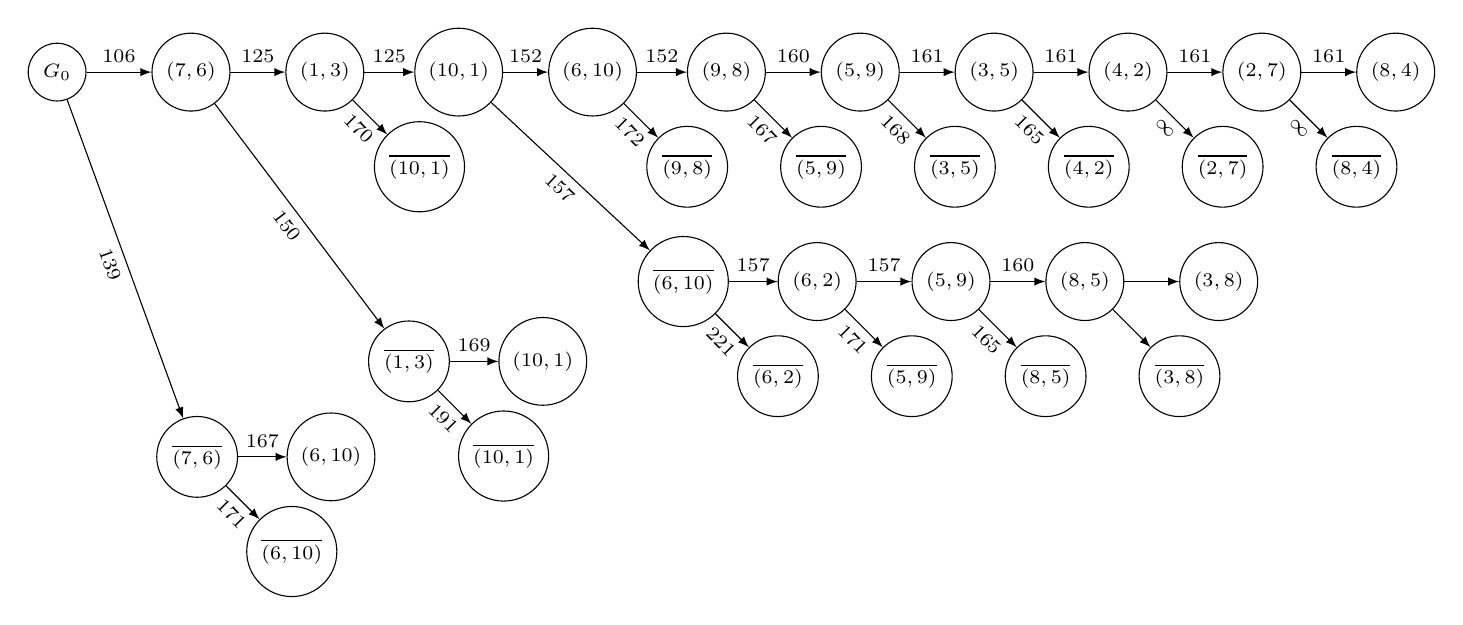
\begin{tikzpicture}[
        grow=east, % Дерево растет слева направо
        level 1/.style = {level distance=1.70cm}, % Расстояние между уровнями
        edge from parent/.style = {draw, -latex},
        kant/.style={text width=2cm, text centered, sloped, font=\scriptsize},
        cell/.style={circle, draw, align=center, font=\scriptsize}, % Стиль узлов
    ]

    \node[cell] {$G_0$}
    child[grow=east] {node[cell] {$(7, 6)$}
            child[grow=east] {node[cell] {$(1, 3)$}
                    child[grow=east] {node[cell] {$(10, 1)$}
                            child[grow=east] {node[cell] {$(6, 10)$}
                                    child[grow=east] {node[cell] {$(9, 8)$}
                                            child[grow=east] {node[cell] {$(5, 9)$}
                                                    child[grow=east] {node[cell] {$(3, 5)$}
                                                            child[grow=east] {node[cell] {$(4, 2)$}
                                                                    child[grow=east] {node[cell] {$(2, 7)$}
                                                                            child[grow=east] {node[cell] {$(8, 4)$} edge from parent node[kant, above] {161}}
                                                                            child[grow=south east] {node[cell] {$\overline{(8, 4)}$} edge from parent node[kant, below] {$\infty$}}
                                                                            edge from parent node[kant, above] {161}}
                                                                    child[grow=south east] {node[cell] {$\overline{(2, 7)}$} edge from parent node[kant, below] {$\infty$}}
                                                                    edge from parent node[kant, above] {161}}
                                                            child[grow=south east] {node[cell] {$\overline{(4, 2)}$} edge from parent node[kant, below] {165}}
                                                            edge from parent node[kant, above] {161}}
                                                    child[grow=south east] {node[cell] {$\overline{(3, 5)}$} edge from parent node[kant, below] {168}}
                                                    edge from parent node[kant, above] {160}}
                                            child[grow=south east] {node[cell] {$\overline{(5, 9)}$} edge from parent node[kant, below] {167}}
                                            edge from parent node[kant, above] {152}}
                                    child[grow=south east] {node[cell] {$\overline{(9, 8)}$} edge from parent node[kant, below] {172}}
                                    edge from parent node[kant, above] {152}}
                            child[grow=317, level distance=3.9cm] {node[cell] {$\overline{(6, 10)}$}
                                    child[grow=east, level distance=1.70cm] {node[cell] {$(6, 2)$}
                                            child[grow=east] {node[cell] {$(5, 9)$}
                                                    child[grow=east] {node[cell] {$(8, 5)$}
                                                            child[grow=east] {node[cell] {$(3, 8)$}}
                                                            child[grow=south east] {node[cell] {$\overline{(3, 8)}$}}
                                                            edge from parent node[kant, above] {160}}
                                                    child[grow=south east] {node[cell] {$\overline{(8, 5)}$} edge from parent node[kant, below] {165}}
                                                    edge from parent node[kant, above] {157}}
                                            child[grow=south east] {node[cell] {$\overline{(5, 9)}$} edge from parent node[kant, below] {171}}
                                            edge from parent node[kant, above] {157}}
                                    child[grow=south east, level distance=1.70cm] {node[cell] {$\overline{(6, 2)}$} edge from parent node[kant, below] {221}}
                                    edge from parent node[kant, below] {157}}
                            edge from parent node[kant, above] {125}}
                    child[grow=south east] {node[cell] {$\overline{(10, 1)}$} edge from parent node[kant, below] {170}}
                    edge from parent node[kant, above] {125}}
            child[grow=307, level distance=4.6cm] {node[cell] {$\overline{(1, 3)}$}
                    child[grow=east, level distance=1.7cm]{node[cell] {$(10, 1)$} edge from parent node[kant, above] {169}}
                    child[grow=south east, level distance=1.7cm]{node[cell] {$\overline{(10, 1)}$} edge from parent node[kant, below] {191}}
                    edge from parent node[kant, below] {150}}
            edge from parent node[kant, above] {106}}
    child[grow=290, level distance=5.2cm] {node[cell] {$\overline{(7, 6)}$}
            child[grow=east, level distance=1.7cm] {node[cell] {$(6, 10)$} edge from parent node[kant, above] {167}}
            child[grow=south east, level distance=1.7cm] {node[cell] {$\overline{(6, 10)}$} edge from parent node[kant, below] {171}}
            edge from parent node[kant, below] {139}};
\end{tikzpicture}

Найдём оценку множества $\overline{(3, 8)}$: $w(\overline{(3, 8)}) = w((8, 5)) + Q_{3, 8} = 160 + 46 = 206$.

Находим оценку множества $(3, 8)$. Для этого нужно вычеркнуть из таблицы строку 3 и столбец 8, а также исключить циклы: поставить $\infty$ в ячейку $(9, 10)$, чтобы не возникло цикла $1 \to 3 \to 8 \to 5 \to 9 \to 10 \to 1$.

\[
    \begin{array}{|>{\columncolor{lightgray}}c|c|c|c|>{\columncolor{LightBlue}}c|}
        \hline \rowcolor{lightgray}
        \text{Город} & 4      & 7  & 10     & \text{min}            \\
        \hline
        2            & 1      & 0  & 4      & 0                     \\
        \hline
        4            & \infty & 0  & 0      & 0                     \\
        \hline
        9            & 18     & 84 & \infty & 18                    \\
        \hline \rowcolor{LightBlue}
        \text{min}   &        &    &        & \cellcolor{Chocolate} \\
        \hline
    \end{array}
\]

Редуцируем таблицу:

\[
    \begin{array}{|>{\columncolor{lightgray}}c|c|c|c|>{\columncolor{LightBlue}}c|}
        \hline \rowcolor{lightgray}
        \text{Город} & 4      & 7  & 10     & \text{min}              \\
        \hline
        2            & 1      & 0  & 4      & 0                       \\
        \hline
        4            & \infty & 0  & 0      & 0                       \\
        \hline
        9            & 0      & 66 & \infty & 18                      \\
        \hline \rowcolor{LightBlue}
        \text{min}   & 0      & 0  & 0      & \cellcolor{Chocolate}18 \\
        \hline
    \end{array}
\]

$h = 18$. Это значит, что $w((3, 8)) = w((8, 5)) + h = 160 + 18 = 178$.

$w(\overline{(3, 8)}) = 206$, $w((3, 8)) = 178$. Заметим, что все они больше полученной нами ранее оценки $w((8, 4)) = 161$. Это значит, что мы можем остановить процесс ветвления для тупиковой ветви $\overline{(6, 10)}$.

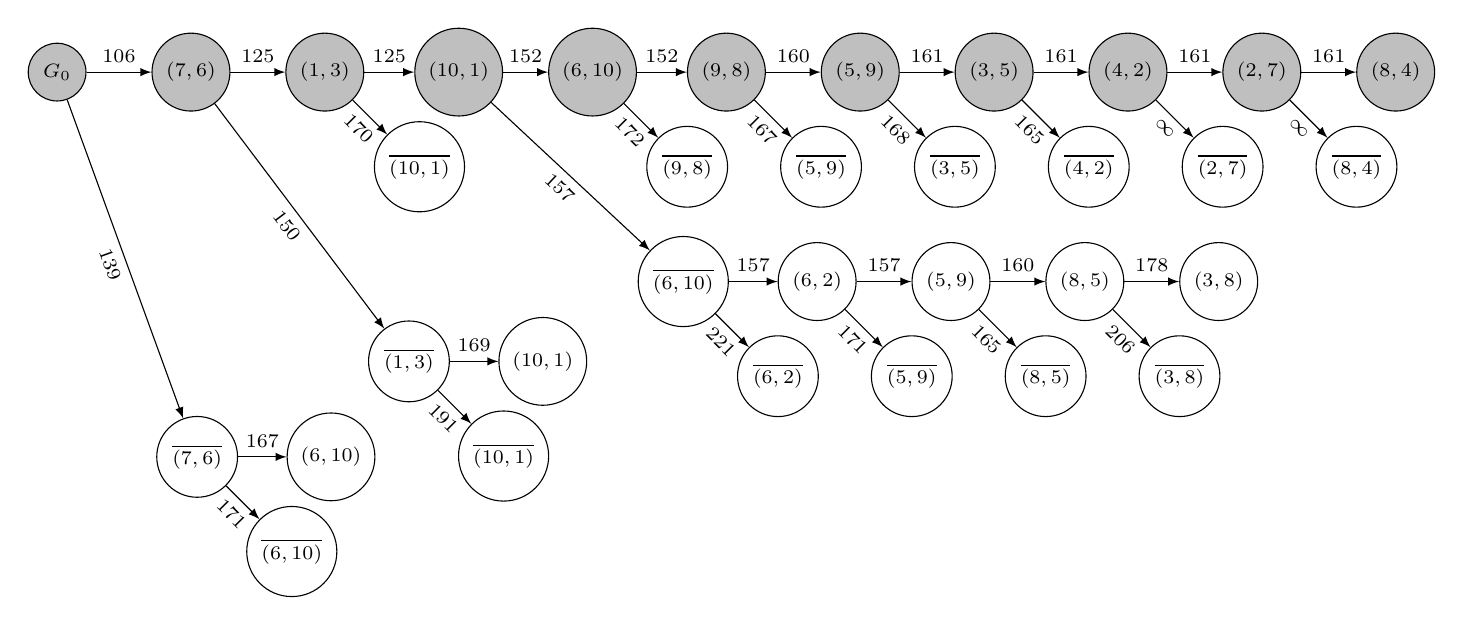
\begin{tikzpicture}[
        grow=east, % Дерево растет слева направо
        level 1/.style = {level distance=1.70cm}, % Расстояние между уровнями
        edge from parent/.style = {draw, -latex},
        kant/.style={text width=2cm, text centered, sloped, font=\scriptsize},
        cell/.style={circle, draw, align=center, font=\scriptsize}, % Стиль узлов
    ]

    \node[cell, fill=lightgray] {$G_0$}
    child[grow=east] {node[cell, fill=lightgray] {$(7, 6)$}
            child[grow=east] {node[cell, fill=lightgray] {$(1, 3)$}
                    child[grow=east] {node[cell, fill=lightgray] {$(10, 1)$}
                            child[grow=east] {node[cell, fill=lightgray] {$(6, 10)$}
                                    child[grow=east] {node[cell, fill=lightgray] {$(9, 8)$}
                                            child[grow=east] {node[cell, fill=lightgray] {$(5, 9)$}
                                                    child[grow=east] {node[cell, fill=lightgray] {$(3, 5)$}
                                                            child[grow=east] {node[cell, fill=lightgray] {$(4, 2)$}
                                                                    child[grow=east] {node[cell, fill=lightgray] {$(2, 7)$}
                                                                            child[grow=east] {node[cell, fill=lightgray] {$(8, 4)$} edge from parent node[kant, above] {161}}
                                                                            child[grow=south east] {node[cell] {$\overline{(8, 4)}$} edge from parent node[kant, below] {$\infty$}}
                                                                            edge from parent node[kant, above] {161}}
                                                                    child[grow=south east] {node[cell] {$\overline{(2, 7)}$} edge from parent node[kant, below] {$\infty$}}
                                                                    edge from parent node[kant, above] {161}}
                                                            child[grow=south east] {node[cell] {$\overline{(4, 2)}$} edge from parent node[kant, below] {165}}
                                                            edge from parent node[kant, above] {161}}
                                                    child[grow=south east] {node[cell] {$\overline{(3, 5)}$} edge from parent node[kant, below] {168}}
                                                    edge from parent node[kant, above] {160}}
                                            child[grow=south east] {node[cell] {$\overline{(5, 9)}$} edge from parent node[kant, below] {167}}
                                            edge from parent node[kant, above] {152}}
                                    child[grow=south east] {node[cell] {$\overline{(9, 8)}$} edge from parent node[kant, below] {172}}
                                    edge from parent node[kant, above] {152}}
                            child[grow=317, level distance=3.9cm] {node[cell] {$\overline{(6, 10)}$}
                                    child[grow=east, level distance=1.70cm] {node[cell] {$(6, 2)$}
                                            child[grow=east] {node[cell] {$(5, 9)$}
                                                    child[grow=east] {node[cell] {$(8, 5)$}
                                                            child[grow=east] {node[cell] {$(3, 8)$} edge from parent node[kant, above] {178}}
                                                            child[grow=south east] {node[cell] {$\overline{(3, 8)}$} edge from parent node[kant, below] {206}}
                                                            edge from parent node[kant, above] {160}}
                                                    child[grow=south east] {node[cell] {$\overline{(8, 5)}$} edge from parent node[kant, below] {165}}
                                                    edge from parent node[kant, above] {157}}
                                            child[grow=south east] {node[cell] {$\overline{(5, 9)}$} edge from parent node[kant, below] {171}}
                                            edge from parent node[kant, above] {157}}
                                    child[grow=south east, level distance=1.70cm] {node[cell] {$\overline{(6, 2)}$} edge from parent node[kant, below] {221}}
                                    edge from parent node[kant, below] {157}}
                            edge from parent node[kant, above] {125}}
                    child[grow=south east] {node[cell] {$\overline{(10, 1)}$} edge from parent node[kant, below] {170}}
                    edge from parent node[kant, above] {125}}
            child[grow=307, level distance=4.6cm] {node[cell] {$\overline{(1, 3)}$}
                    child[grow=east, level distance=1.7cm]{node[cell] {$(10, 1)$} edge from parent node[kant, above] {169}}
                    child[grow=south east, level distance=1.7cm]{node[cell] {$\overline{(10, 1)}$} edge from parent node[kant, below] {191}}
                    edge from parent node[kant, below] {150}}
            edge from parent node[kant, above] {106}}
    child[grow=290, level distance=5.2cm] {node[cell] {$\overline{(7, 6)}$}
            child[grow=east, level distance=1.7cm] {node[cell] {$(6, 10)$} edge from parent node[kant, above] {167}}
            child[grow=south east, level distance=1.7cm] {node[cell] {$\overline{(6, 10)}$} edge from parent node[kant, below] {171}}
            edge from parent node[kant, below] {139}};
\end{tikzpicture}

Итак, критерий оптимальности для задачи коммивояжёра выполнен. Оптимальный маршрут: $1 \to 3 \to 5 \to 9 \to 8 \to 4 \to 2 \to 7 \to 6 \to 10 \to 1$.
По расчётам получаем, что длина оптимального маршрута равна 161. Давайте это проверим по изначальной таблице:

\[
    \begin{array}{|>{\columncolor{lightgray}}c|c|c|c|c|c|c|c|c|c|c|}
        \hline \rowcolor{lightgray}
        \text{Город} & 1                               & 2                              & 3                              & 4                             & 5                              & 6                             & 7                             & 8                              & 9                              & 10                            \\
        \hline
        1            & \infty                          & 92                             & \mycellcolor\doublecell{14}{1} & 71                            & 60                             & 20                            & 82                            & 86                             & 74                             & 74                            \\
        \hline
        2            & 87                              & \infty                         & 23                             & 2                             & 21                             & 52                            & \mycellcolor\doublecell{1}{7} & 87                             & 29                             & 37                            \\
        \hline
        3            & 1                               & 63                             & \infty                         & 20                            & \mycellcolor\doublecell{32}{2} & 75                            & 57                            & 21                             & 88                             & 48                            \\
        \hline
        4            & 90                              & \mycellcolor\doublecell{58}{6} & 41                             & \infty                        & 59                             & 79                            & 14                            & 61                             & 61                             & 46                            \\
        \hline
        5            & 61                              & 50                             & 54                             & 63                            & \infty                         & 100                           & 50                            & 6                              & \mycellcolor\doublecell{20}{3} & 72                            \\
        \hline
        6            & 38                              & 17                             & 3                              & 88                            & 59                             & \infty                        & 8                             & 89                             & 52                             & \mycellcolor\doublecell{1}{9} \\
        \hline
        7            & 83                              & 91                             & 59                             & 70                            & 43                             & \mycellcolor\doublecell{7}{8} & \infty                        & 34                             & 77                             & 80                            \\
        \hline
        8            & 35                              & 49                             & 3                              & \mycellcolor\doublecell{1}{5} & 5                              & 53                            & 3                             & \infty                         & 92                             & 62                            \\
        \hline
        9            & 17                              & 89                             & 43                             & 33                            & 73                             & 61                            & 99                            & \mycellcolor\doublecell{13}{4} & \infty                         & 47                            \\
        \hline
        10           & \mycellcolor\doublecell{14}{10} & 71                             & 77                             & 86                            & 61                             & 39                            & 84                            & 79                             & 81                             & \infty                        \\
        \hline
    \end{array}
\]

$ 14 + 32 + 20 + 13 + 1 + 58 + 1 + 7 + 1 + 14 = 161$.

В конце приведём сравнение с программным решением (код можно найти \href{https://github.com/retrobannerS/optimization_methods/blob/main/python/07-lab/salesman.ipynb}{здесь}) задачи коммивояжёра:

\begin{longtable}[]{@{}|llll|@{}}
    \toprule\noalign{}
      & результат & путь                                & шагов \\
    \midrule\noalign{}
    \endhead
    \bottomrule\noalign{}
    \endlastfoot
    0 & 161.0     & {[}7, 6, 10, 1, 3, 5, 9, 8, 4, 2{]} & 62    \\
\end{longtable}

Таким образом путь можно перевести в матрицу $X = \|x_{ij}\|$, где в $x_{ij} = 1$ стоит, если оптимально ехать из города $i$ в город $j$ иначе $X_{ij} = 0$.

\[
    X = \begin{pmatrix}
        0 & 0 & 1 & 0 & 0 & 0 & 0 & 0 & 0 & 0 \\
        0 & 0 & 0 & 0 & 0 & 0 & 1 & 0 & 0 & 0 \\
        0 & 0 & 0 & 0 & 1 & 0 & 0 & 0 & 0 & 0 \\
        0 & 1 & 0 & 0 & 0 & 0 & 0 & 0 & 0 & 0 \\
        0 & 0 & 0 & 0 & 0 & 0 & 0 & 0 & 1 & 0 \\
        0 & 0 & 0 & 0 & 0 & 0 & 0 & 0 & 0 & 1 \\
        0 & 0 & 0 & 0 & 0 & 1 & 0 & 0 & 0 & 0 \\
        0 & 0 & 0 & 1 & 0 & 0 & 0 & 0 & 0 & 0 \\
        0 & 0 & 0 & 0 & 0 & 0 & 0 & 1 & 0 & 0 \\
        1 & 0 & 0 & 0 & 0 & 0 & 0 & 0 & 0 & 0 \\
    \end{pmatrix}
\]

\textbf{Ответ:} $\min F = 161$, оптимальный путь: $1 \to 3 \to 5 \to 9 \to 8 \to 4 \to 2 \to 7 \to 6 \to 10 \to 1$. \label{07-lab-answer}

